\chapter{A Novel Implementation of the \glsentryshort{lartpc} Technology}
\label{chap:ac}

While the theory and improvements of individual \lartpc{} subsystems were discussed in Chapter~\ref{chap:studies}, this chapter presents the amalgamation of all my findings into a new \lartpc{} concept, \AC{}, aligned to the needs of future \lartpc{} neutrino detectors.
The results of the \AC{} pixel demonstrator are presented, alongside a reconstruction framework I developed, yielding fully reconstructed \gls{3d} cosmic muon tracks.
Both have been published in~\cite{pixel_paper, pixel_proceedings}.
Afterwards, the \AC{} modular \lartpc{} concept is introduced.


\section{\AC{} Pixel Demonstrator}
\label{sec:ac_viper}

This section describes the results obtained from the pixel demonstrator for the \AC{} project (see Chapter~\ref{sec:ac_argoncube}).
A particular focus is put on the reconstruction of the recorded cosmic ray events.
 
The pixelated anode plane, shown in Figure~\ref{fig:viper_pixies}, was produced as a conventional \gls{pcb}.
It implements the \gls{roi}-based analogue multiplexing scheme introduced in Section~\ref{sec:studies_pixel-ro}.
The pixelated area is \SI{100}{\milli\metre} across, the pixels are formed of \SI{900}{\micro\metre} vias with a pitch of \SI{2.54}{\milli\metre}.
An inductive focusing grid surrounds the pixels, it is made from \SI{152.4}{\micro\metre} copper traces split into 28 regions.
There are \num{6 x 6} pixels per region, giving a total of 1008 pixels. 

\begin{figure}[tbp]
	\centering
	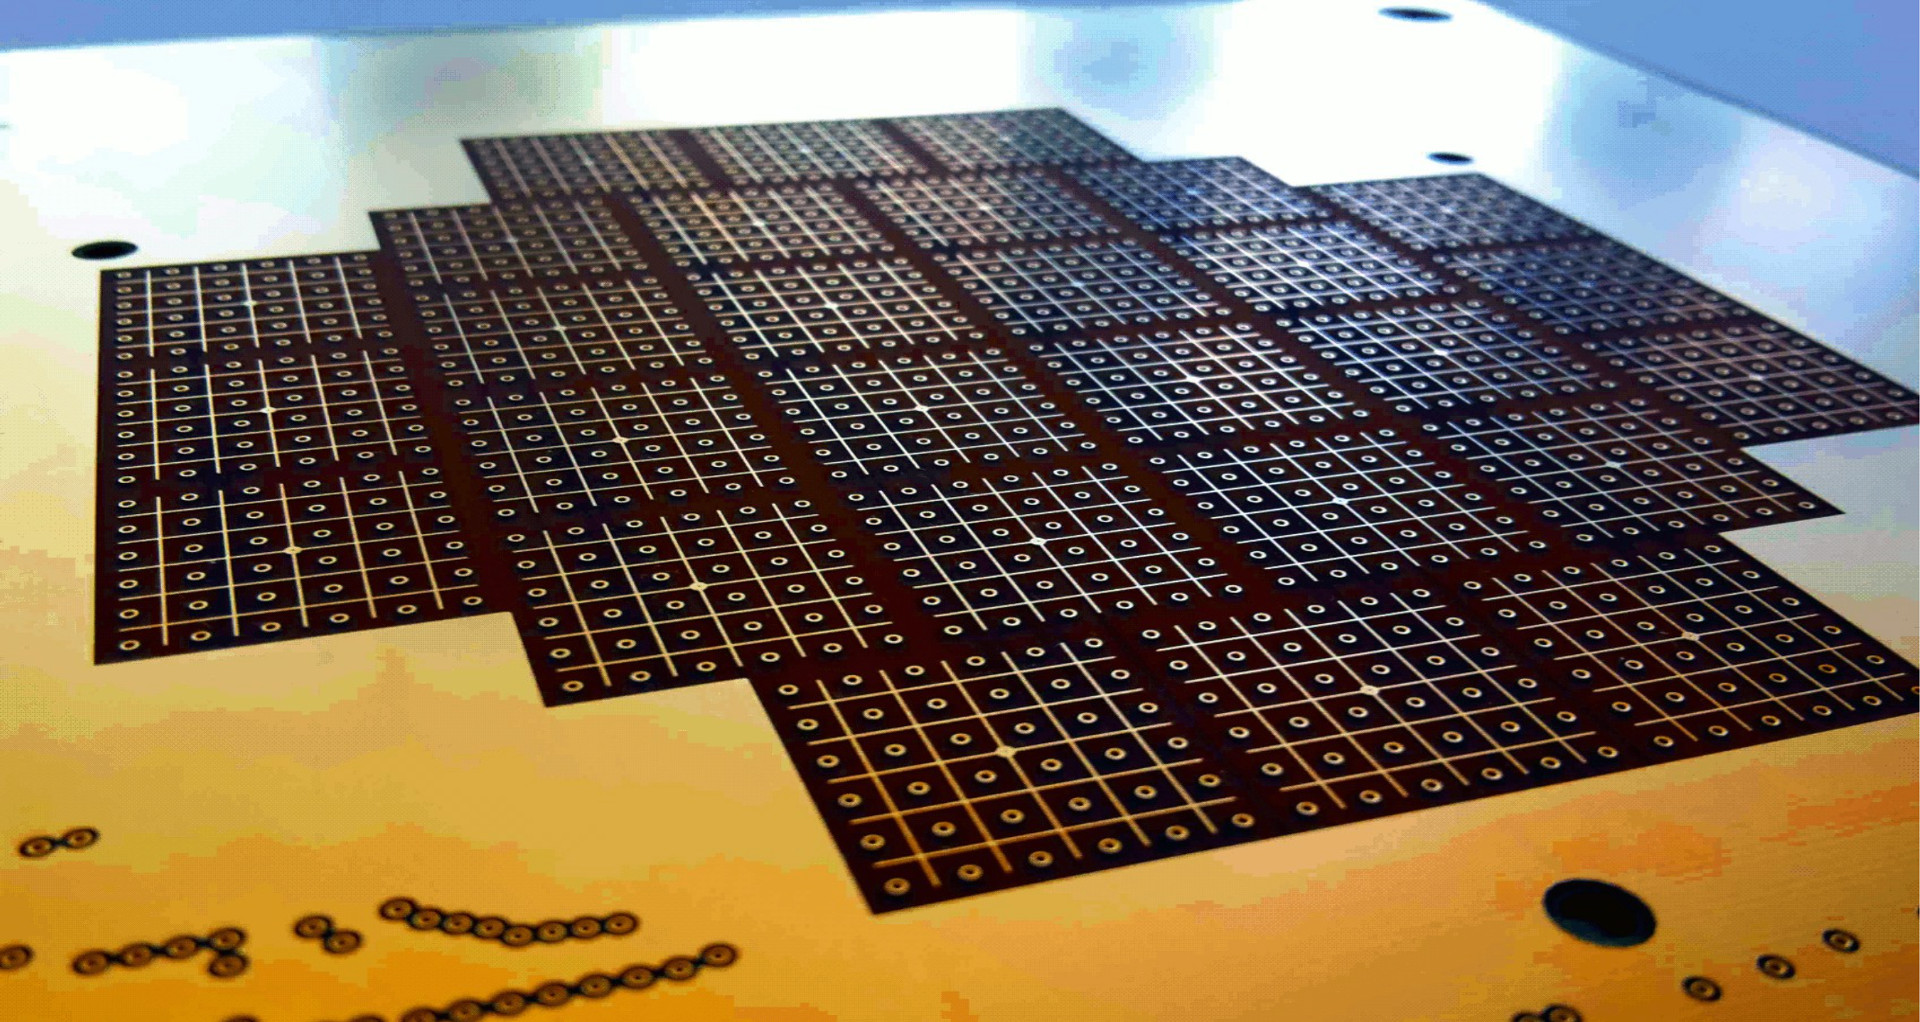
\includegraphics[width=\textwidth]{viper/pixies}
	\caption[Pixel demonstrator readout plane]{%
		First (high-capacitance) version of the pixelated anode \acrshort{pcb}.
		The pixelated readout area is \SI{100}{\milli\metre} in diameter.
		Each charge collection pixel is a \SI{900}{\micro\metre} via, at a pitch of \SI{2.54}{\milli\metre}.
		Inductive focusing grids formed of \SI{152.4}{\micro\metre} copper traces surround the pixels.
		There are \num{28} inductive focusing grids with \num{36} pixels per region, a total of \num{1008} pixels.
	}
	\label{fig:viper_pixies}
\end{figure}

Vias were used for pixels instead of pads in order to minimise capacitance.
As detailed in Section~\ref{sec:studies_electronics}, it is important to minimise capacitance of a charge readout.
To further minimise parasitic capacitances the \gls{pcb} design was optimised by removing unnecessary ground planes, routing signal tracks outside necessary ground planes, and increasing the thickness of the \gls{pcb} to \SI{3.5}{\milli\metre} from an initial \SI{1.75}{\milli\metre}. 
The resulting capacitance at each pixel is $\approx \SI{65}{\pico\farad}$ (see Section~\ref{sec:studies_at-ro}).

The pixels are directly connected to the preamplifiers while the inductive focusing grids are decoupled via \SI{10}{\nano\farad} capacitors.
Additionally, the bias voltage is filtered at the input by another \SI{10}{\nano\farad} and \SI{10}{\mega\ohm}.
The full schematic of the bias circuit is depicted in Figure~\ref{fig:viper_pcb_schematic}.

\begin{figure}[tbp]
	\centering
	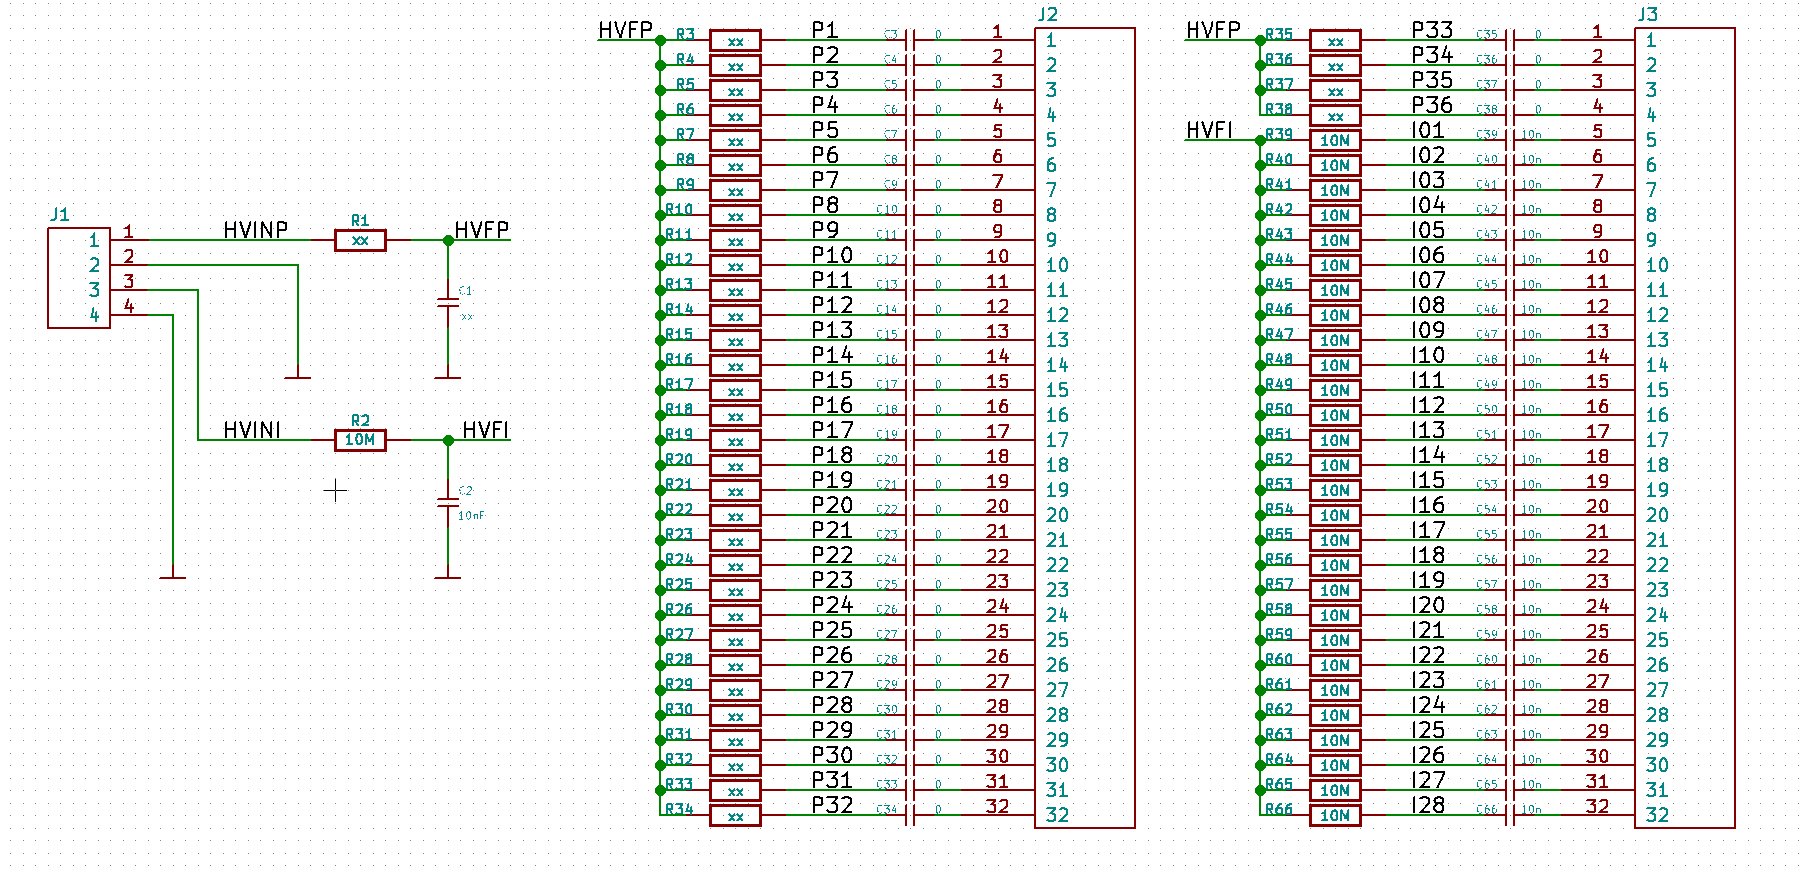
\includegraphics[width=\textwidth]{viper/pixel_pcb_schematic}
	\caption[Pixel demonstrator bias circuit]{%
		Schematic of the bias circuit for the \AC{} pixel demonstrator \acrshort{pcb}.
		On the left the pin header connected to the bias \acrshort{hv} power supply is shown. In the middle and on the right are the connections to the pixels and inductive \acrshort{roi} grids.
		The connections to the preamplifier inputs are located at the positions of labels P1--P36 (pixels) and I1--I28 (\acrshortpl{roi}).
		For simplicity and universality the same circuit was used for both pixels and \acrshortpl{roi} even though only the inductive \acrshort{roi} grids were biased for the measurements described here.
		Therefore, the \acrshortpl{roi} are connected as depicted (R2 and R39--R66, C2 and C39--C66).
		The pixels are directly connected to the preamplifiers by leaving R3--R38 unpopulated and replacing C3--C38 by \SI{0}{\ohm} resistors because no pixel bias is needed.
		Additionally, R1 is \SI{0}{\ohm} and C1 unpopulated, and all unused \acrshort{pcb} traces are grounded by connecting pin 1 of J1 to ground.
	}
	\label{fig:viper_pcb_schematic}
\end{figure}

The bias on the inductive focusing grids has to be sufficient to allow full charge transparency (all charge collected by the pixels), yet low enough to minimise any risk of damaging the cold coupling capacitors.
It was increased incrementally until transparency was observed at \SI{300}{\volt}. 
Simulations suggest this was only \SI{95}{\percent} transparency, with \SI{100}{\percent} at \SI{350}{\volt} (see Figure~\ref{fig:viper_transparency}).
The simulations available at the time of the measurement contained a bug resulting in an underestimation of the bias voltage required for full transparency.
During the measurements the bug became apparent and full transparency had to be estimated by looking at live data from the detector.
Due to the limited accuracy of this method measurements were not taken up to the bias voltage for full transparency suggested by the (corrected) simulation.~\cite{francypants}

The pixel demonstrator \gls{tpc}, shown in Figures~\ref{fig:viper_cad}~and~\ref{fig:viper_v1per}, is cylindrical with an inner diameter of \SI{101}{\milli\metre} and a \SI{590}{\milli\metre} drift length. 
The \gls{tpc} operated with a drift field of \SI{1}{\kilo\volt\per\centi\metre}, corresponding to a total drift time of \SI{281}{\micro\second} at \SI{2.1}{\milli\metre\per\micro\second}~\cite{protoLASER}.

\begin{figure}[tbp]
	\centering
	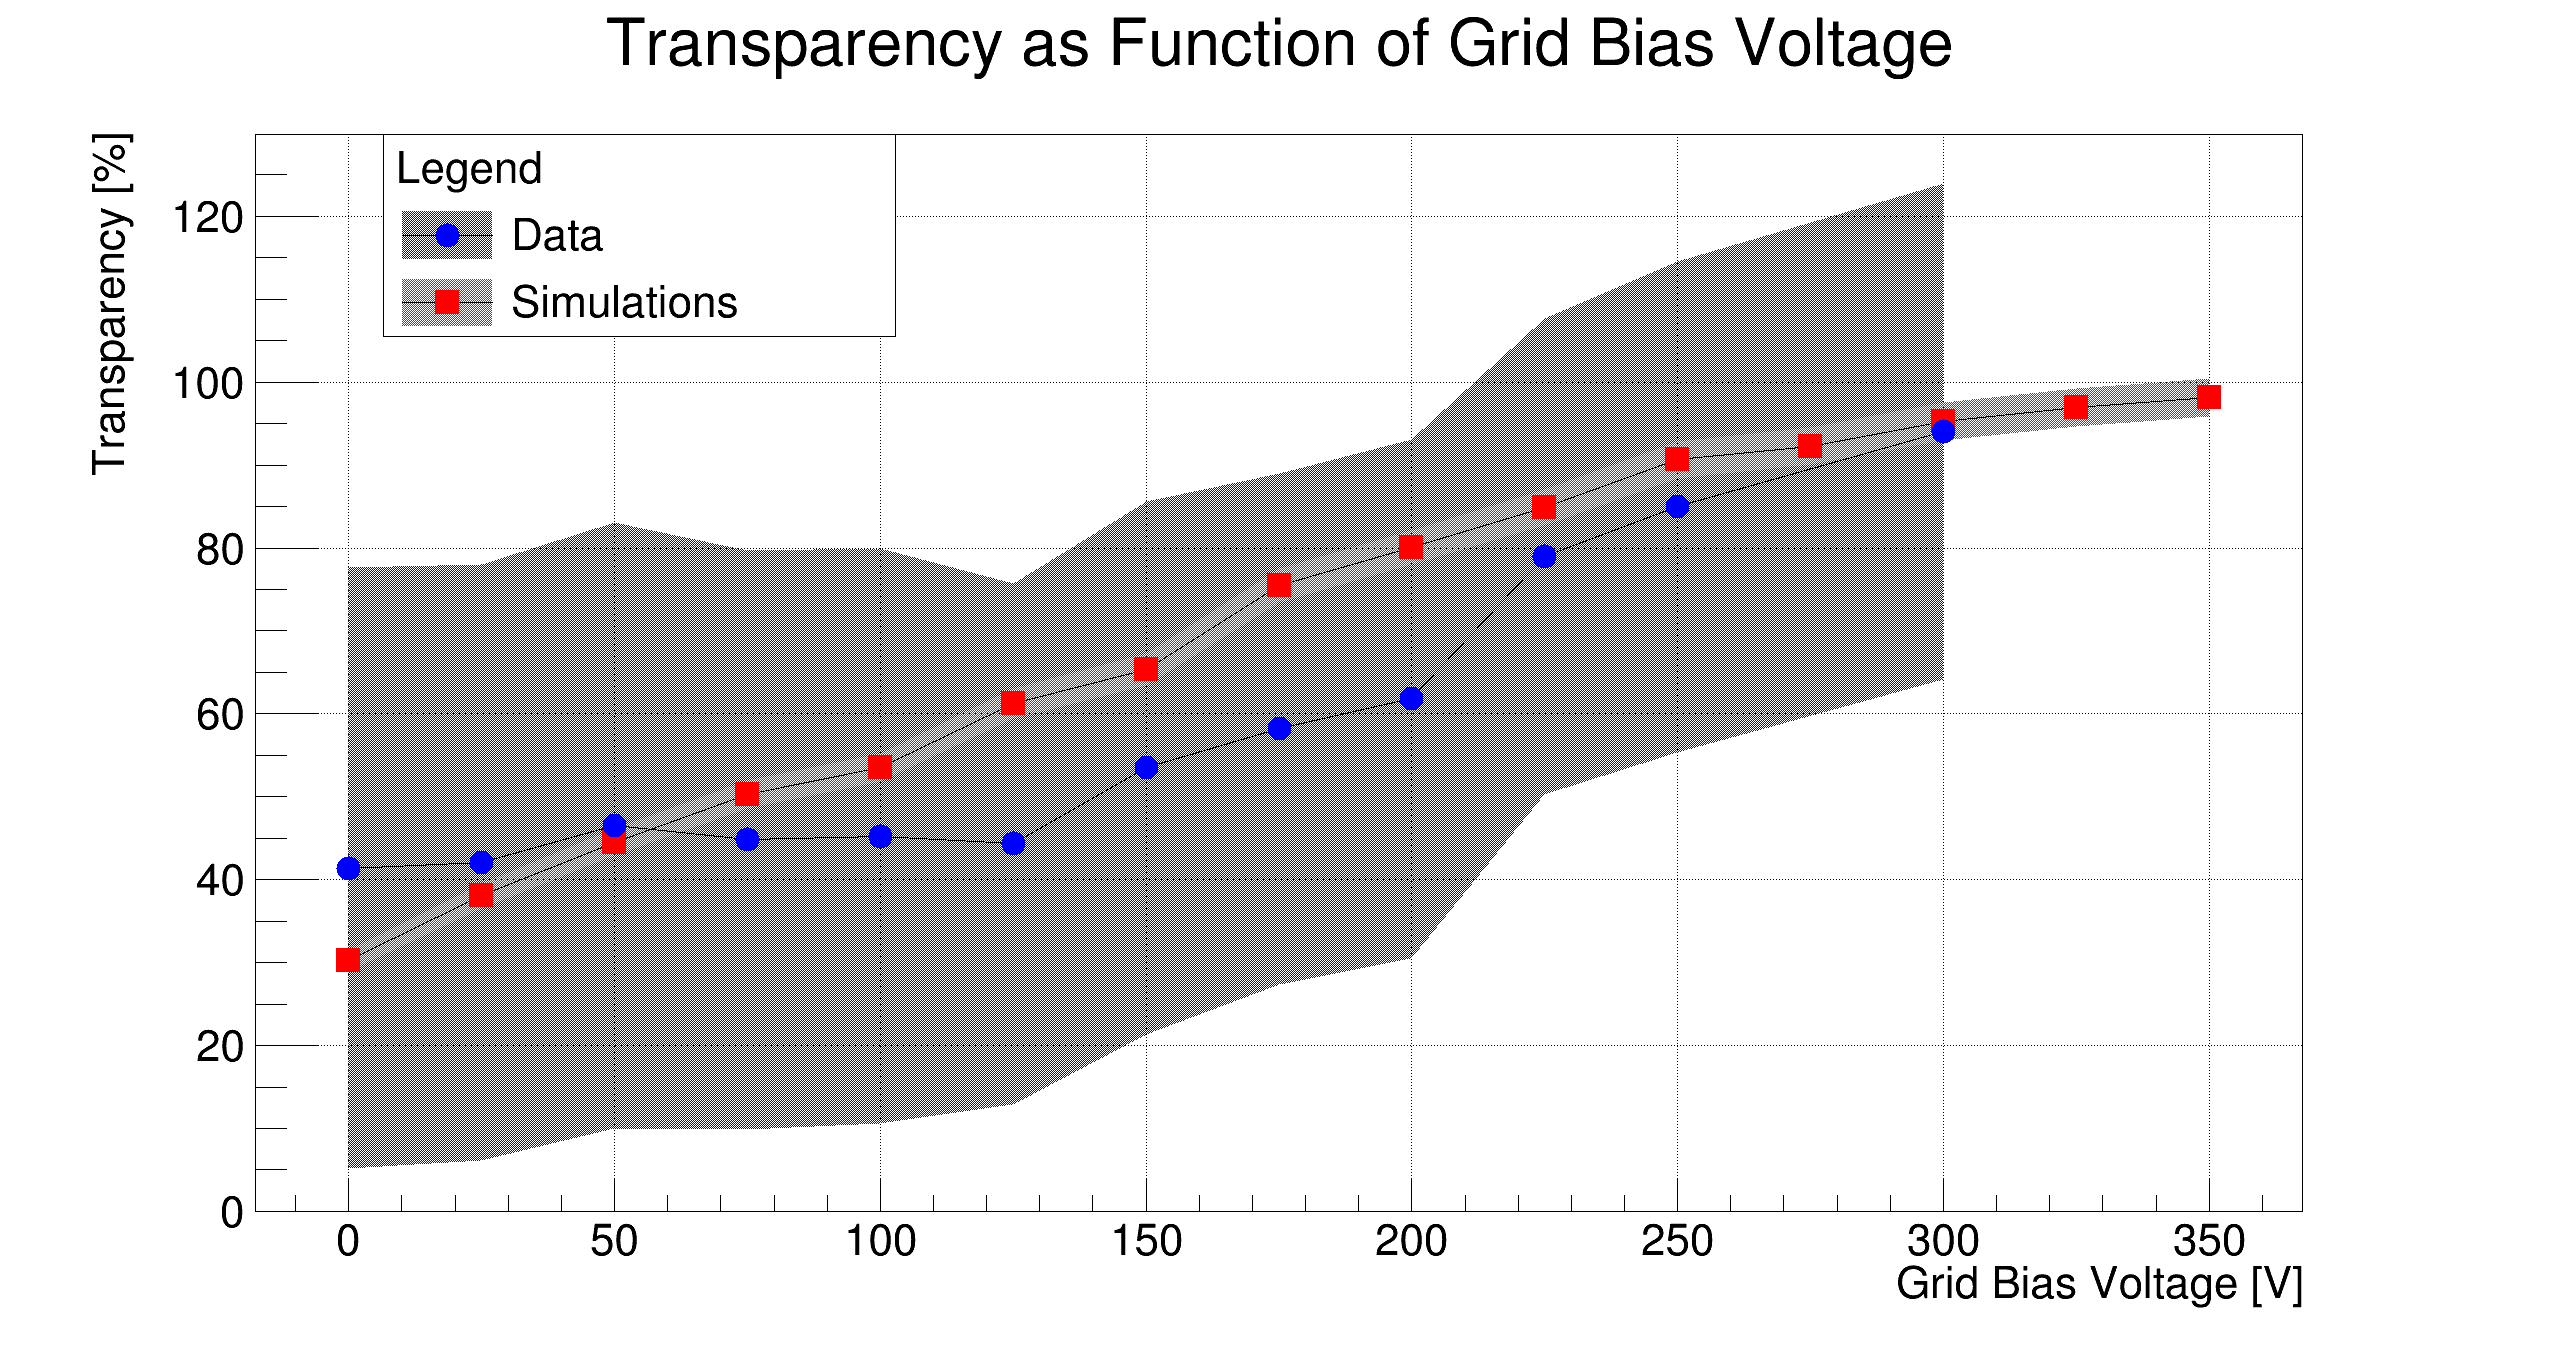
\includegraphics[width=\textwidth]{viper/transparency}
	\caption[Pixel demonstrator charge readout transparency]{%
		Measured and simulated transparency versus bias voltage of the \AC{} pixel demonstrator.~\cite{francypants}
	}
	\label{fig:viper_transparency}
\end{figure}

The field-cage consists of aluminium rings supported by clear acrylic rings, with a cathode formed of a brass disc. 
The dimensions of the field-cage and cathode are shown in Figure~\ref{fig:viper_cad}.
Alternating acrylic rings are split to allow for the circulation of purified \lar{} within the \gls{tpc} volume.
Four square section \gls{pai} uprights support the cathode and field cage, with \gls{peek} screws fixing the pillars to the acrylic rings.
The four \gls{pai} uprights connect to a \gls{pai} frame which supports the anode plane and the light readout \glspl{sipm}, see Figure~\ref{fig:viper_v1per}.   

The resistive divider consists of a chain of \SI{100}{\mega\ohm} \emph{Vishay ROX100100MFKEL} metal oxide resistors~\cite{vishay}.
Each resistor is soldered to its neighbour and fixed to the field cage at each joint with an M3 screw.   

\begin{figure}[tbp]
	\centering
	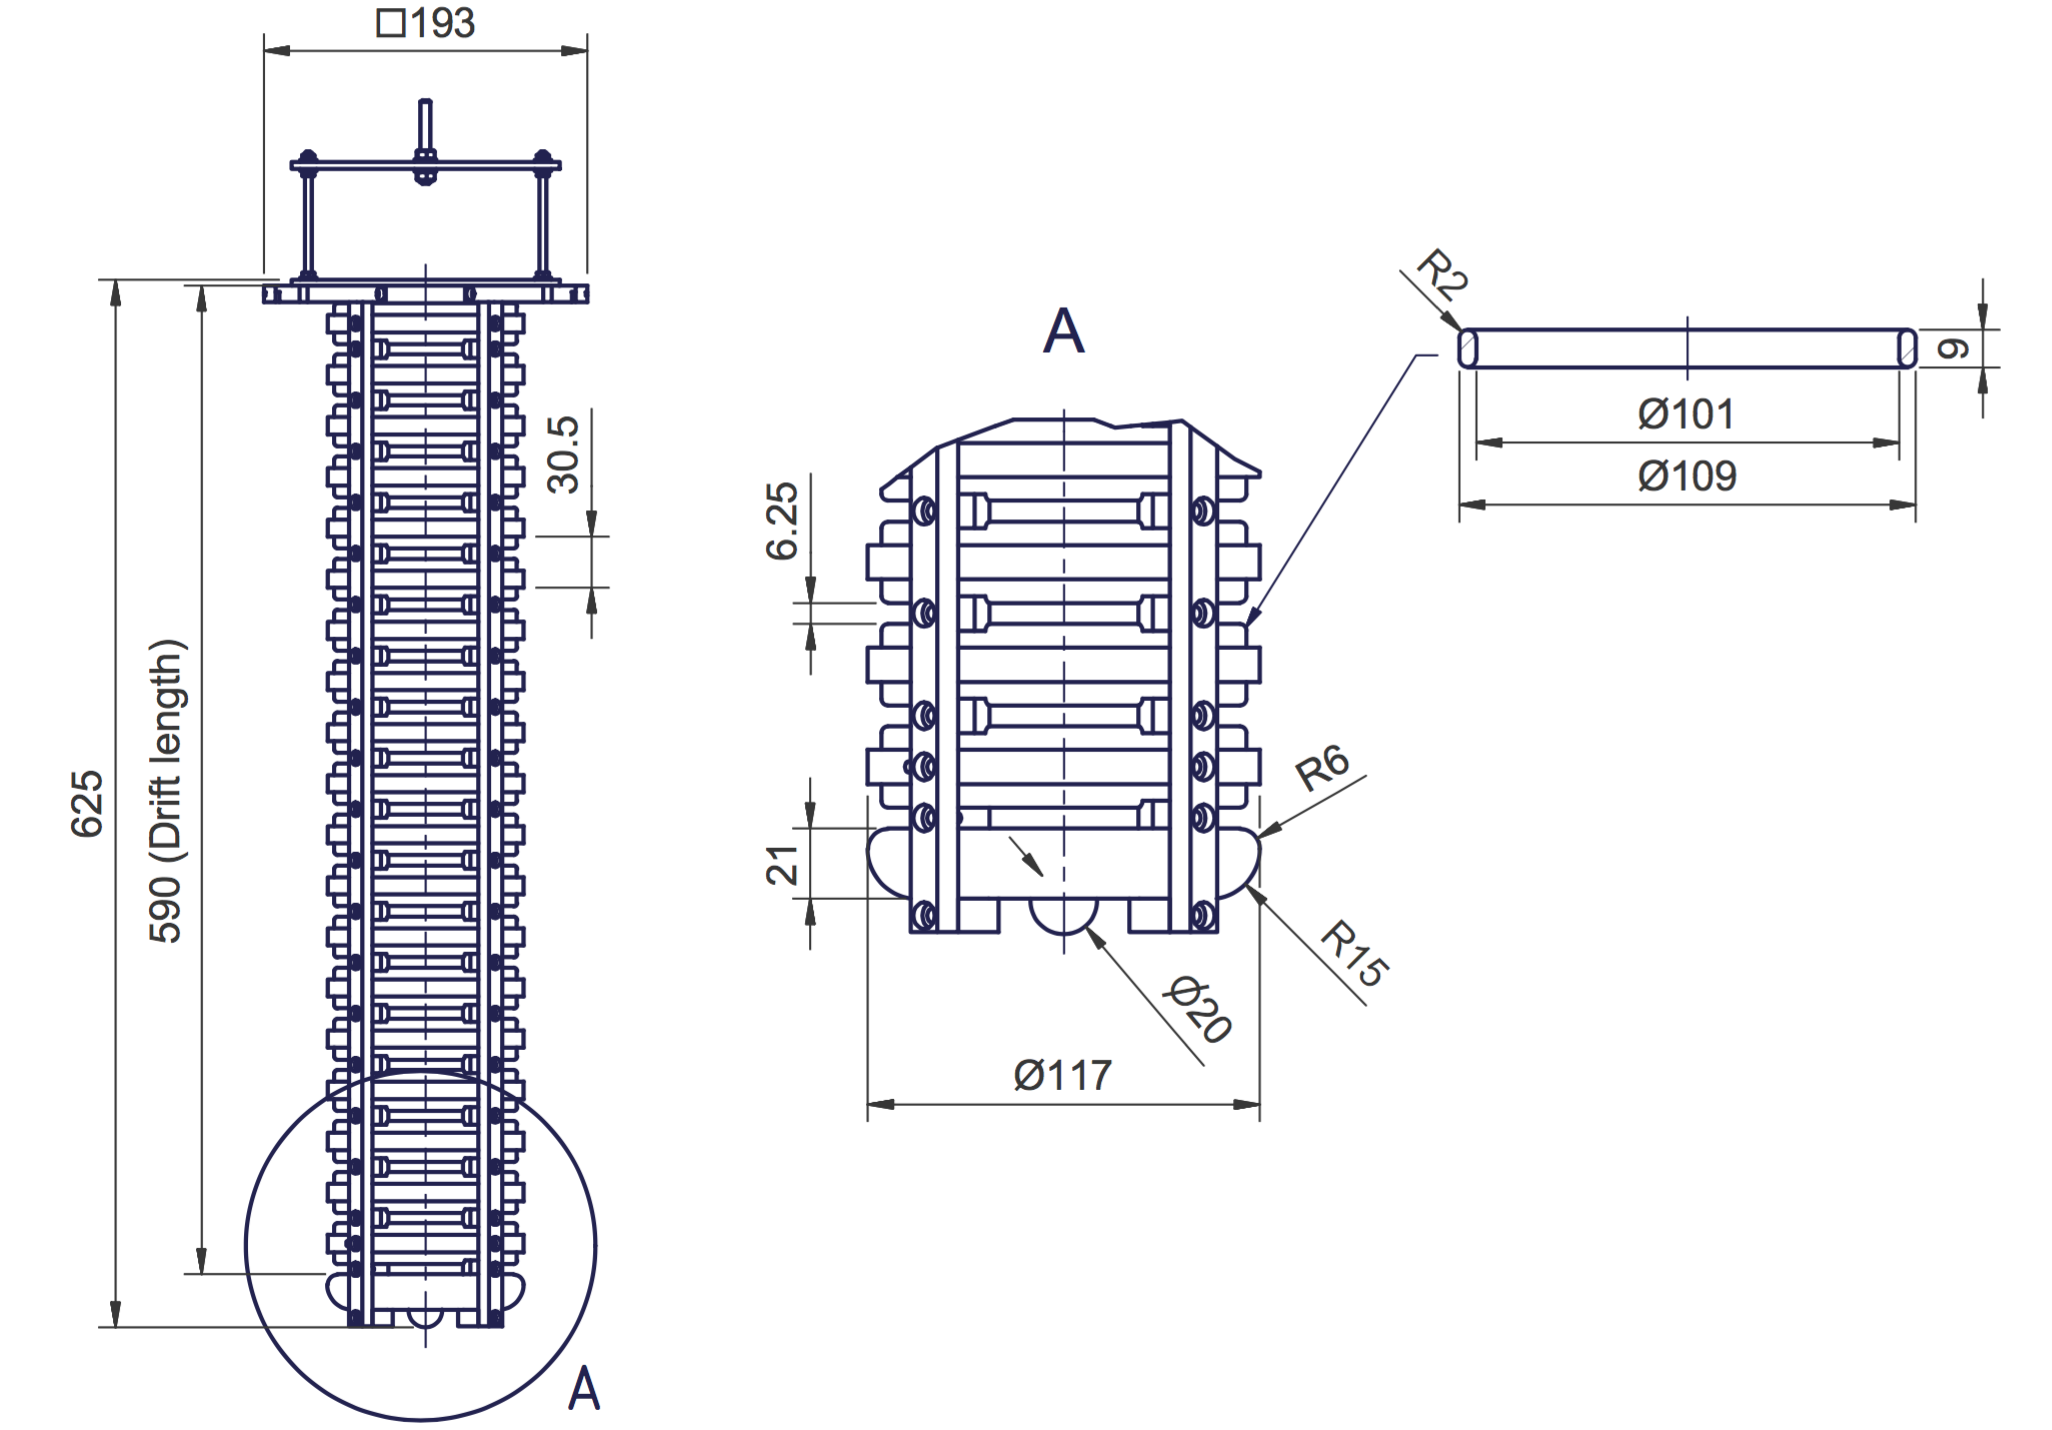
\includegraphics[width=\textwidth]{viper/tpc_cad}
	\caption[Engineering drawing of pixel demonstrator \glsentryshort{tpc}]{%
		Engineering drawing of the pixel demonstration \acrshort{tpc}; \SI{590}{\milli\metre} drift length; \SI{6.25}{\milli\metre} field cage spacing; \SI{101}{\milli\metre} internal diameter.
	}
	\label{fig:viper_cad}
\end{figure}

The acrylic rings provide the light collection; their inner surfaces are machine-polished and coated with the \gls{wls} \gls{tpb}. 
\SI{1}{\milli\metre} diameter \gls{wls} fibres couple the acrylic rings to four \glspl{sipm} mounted close to the anode (see Figure~\ref{fig:viper_v1per}). 
The \glspl{sipm} and their front-end electronics were adapted from those developed at \gls{help} for the \glspl{crt} used in \uboone{} and \sbnd{}~\cite{crt, crt_feb}.
A more detailed description of the light readout system is given in Section~\ref{sec:studies_viper-light-ro}.

The pixel demonstration \gls{tpc} is housed in a double-bath vacuum-insulated cryostat with the outer bath open to atmosphere.
A diameter of \SI{50}{\centi\metre} and a height of \SI{110}{\centi\metre} give an inner volume of $\approx \SI{200}{\litre}$ of \lar{}.
This is the same cryostat that was used for the \gls{hv} studies described in Section~\ref{sec:studies_breakdown}.
The \lar{} filtering method is the same as described in~\cite{2photonAbs}, with \lar{} filtered first on filling through a pair of Oxysorb-Hydrosorb filters, and then recirculated through a single custom-made filter containing both activated copper and silica gel.
\lar{} purity is estimated to be in accordance with~\cite{2photonAbs}, with impurity concentrations $\sim{\SI{1}{ppb}}$ of oxygen-equivalent, which corresponds to a charge lifetime of \SI{290+-30}{\micro\second}.

\begin{figure}[tbp]
	\centering
	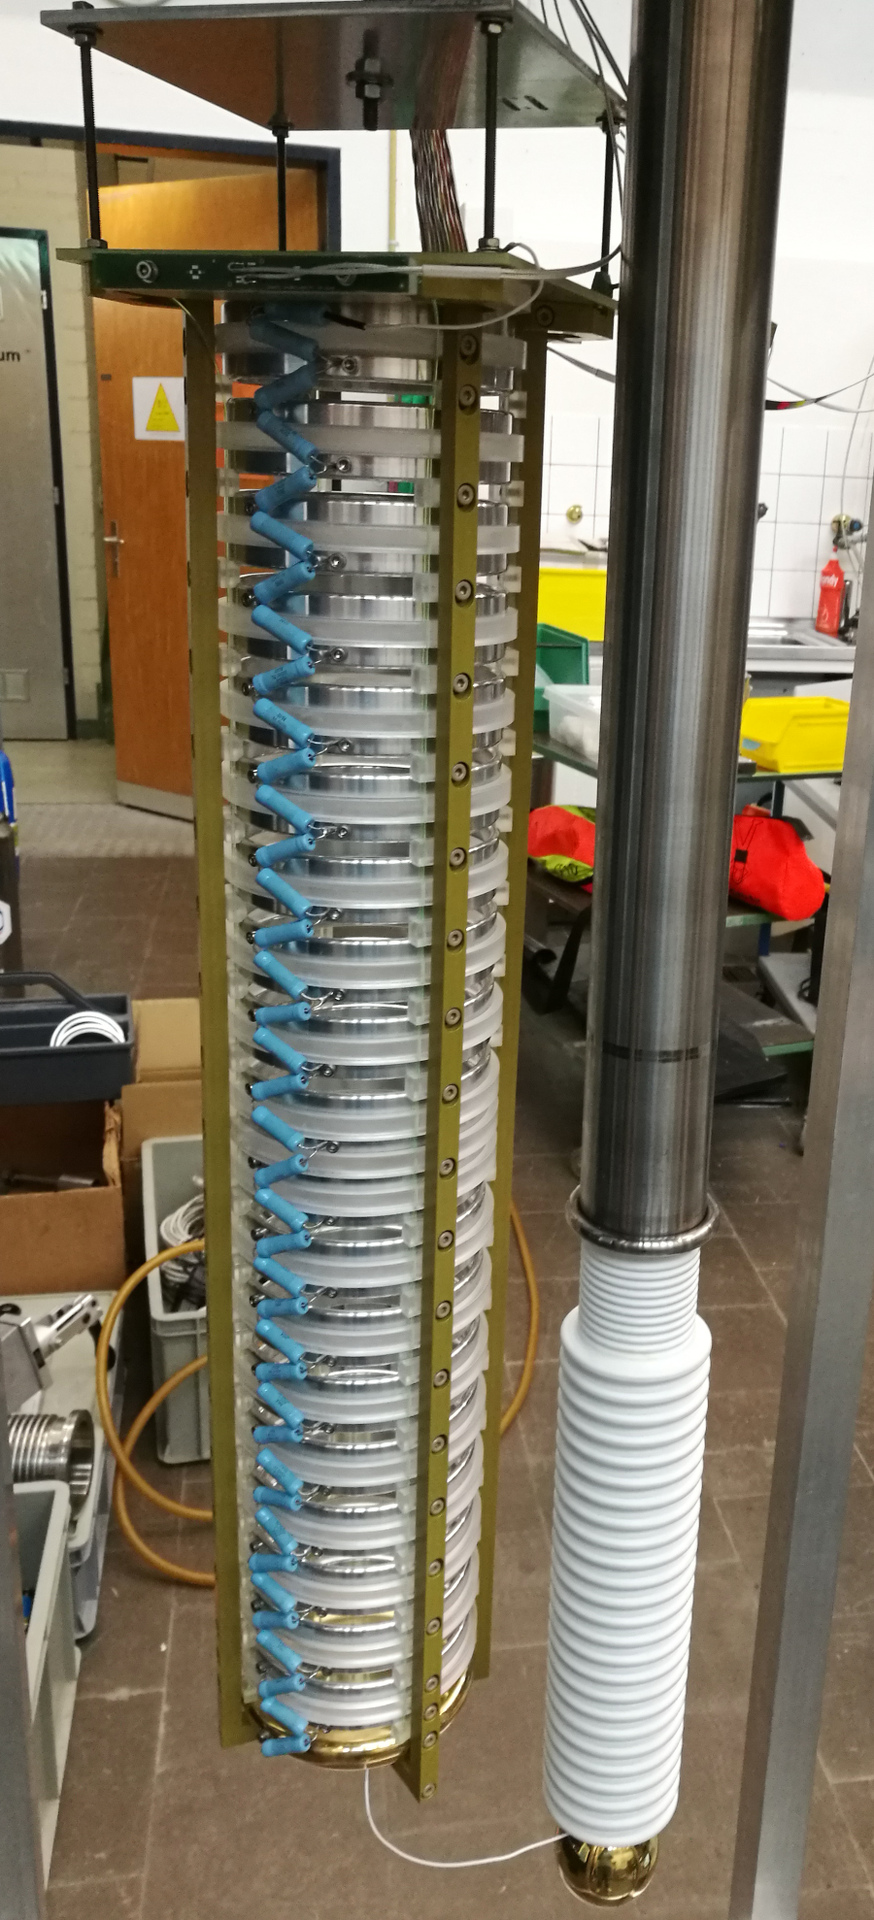
\includegraphics[height=.45\textheight]{viper/viper_original}
	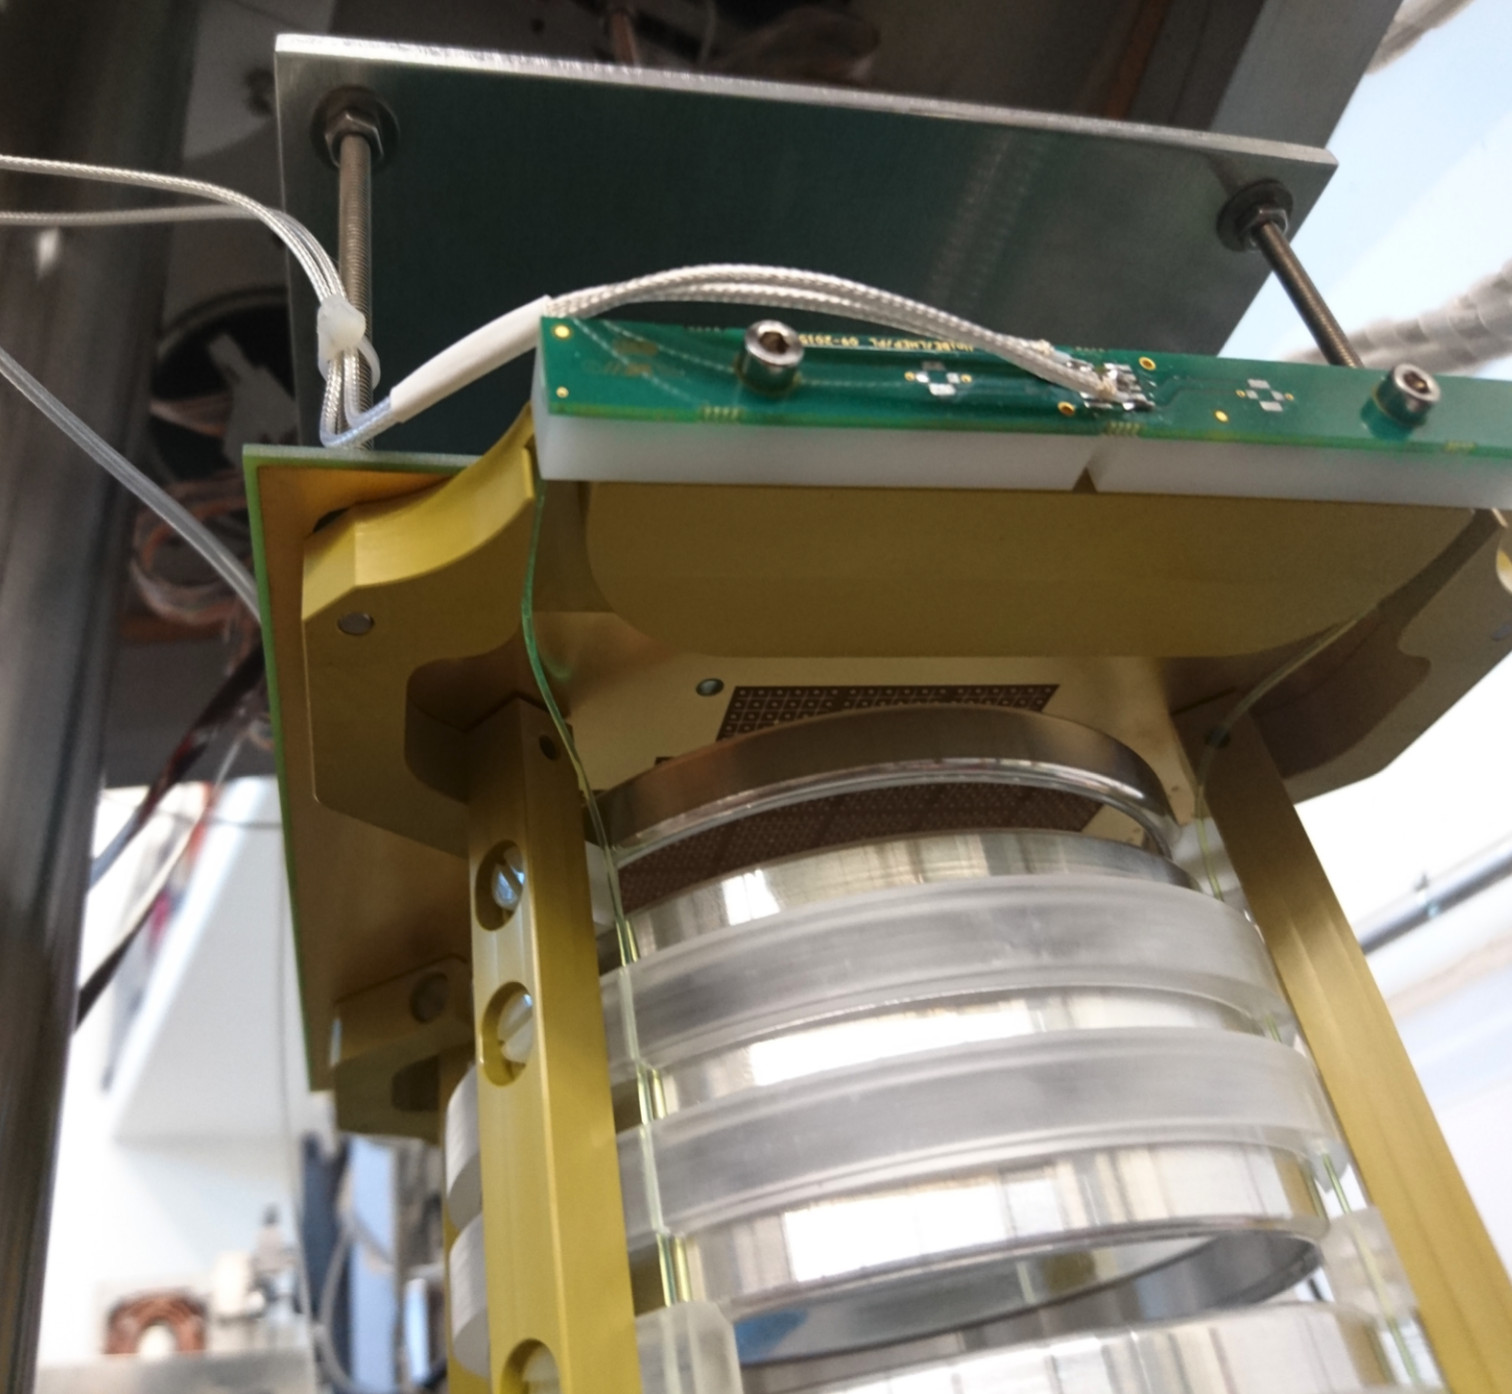
\includegraphics[height=.45\textheight]{viper/viper_sipm}
	\caption[Pixel demonstrator close-up]{%
		Left: Photograph of the  pixel demonstrator \acrshort{tpc} at \acrshort{help}, with the \acrshort{hv} feedthrough.
		Right: Close-up of the light collection system, showing \acrshort{wls} fibres coupling the \acrshortpl{sipm} to the \acrshort{tpb}-coated light guides.
	}
	\label{fig:viper_v1per}
\end{figure}

The \gls{petc} \gls{hv} feedthrough capable of potentials as high as \SI{-130}{\kilo\volt} remains unchanged from the breakdown studies (Section~\ref{sec:studies_breakdown}).
I added a low-pass filter between the power supply and feedthrough, which consists of an \SI{800}{\pico\farad} decoupling capacitor grounded between two \SI{100}{\mega\ohm} resistors connected in series; i.e.\ a \gls{rc} low-pass filter with an additional protection resistor at the output.
For proper insulation the filter circuit is submerged in transformer oil.

Dedicated noise data was taken to assess the \gls{snr}, employing a \SI{5}{\hertz} random trigger.
Drift, focusing, and \gls{sipm} bias voltages were turned off for these measurements.
The data of \num{5000} events was combined.
Subsequently, all pixel and \gls{roi} channels were combined separately and filled into respective amplitude distribution histograms.
Finally, the standard deviation of the noise was calculated by fitting a Gaussian to the amplitude distribution.
This value was used to calculate the \gls{snr} for pixel and \gls{roi} channels according to
\begin{IEEEeqnarray}{rCl}
	\m{\glsentryshort{snr}} & = & \frac{S}{\sigma} \qc
	\label{eq:viper_snr}
\end{IEEEeqnarray}
where $S$ is the signal and $\sigma$ is the noise standard deviation from the Gaussian fit.
As can be seen in the top plot in Figure~\ref{fig:viper_unfilteredRawData} (and also~\ref{fig:electronics_noise-run2}), one of the pixel channels is significantly noisier in comparison to the others, likely caused by a broken preamplifier.
Therefore, this channel was blinded for the \gls{snr} calculations.
The resulting equivalent noise charge is \SI{1095}{\elementarycharge} for the pixel channels and \SI{982}{\elementarycharge} for the inductive \gls{roi} channels.
The noise amplitude distributions are shown in Figure~\ref{fig:electronics_noise-run2}.

\begin{table}[tbp]
	\centering
	\caption[Pixel demonstrator \glsentryshort{snr}]{%
		\acrshort{snr} values obtained from Equation~\eqref{eq:viper_snr}.
		The signal was calculated from theory assuming a \acrshort{mip} at the readout plane or cathode, respectively.
		The average equivalent noise charge was obtained from measurements for pixel and \acrshort{roi} channels, respectively.
	}
	\label{tab:viper_snr}
	\begin{tabu} to \textwidth {llS}
		\toprule
		Channel &			\acrshort{mip} at &	{\acrshort{snr}} \\
		\midrule
		Pixel &				Readout plane &		14 \\
		Pixel &				Cathode &			5.5 \\
		\acrshort{roi} &	Readout plane &		16 \\
		\acrshort{roi} &	Cathode &			6.1 \\
		\bottomrule
	\end{tabu}
\end{table}

The signal $S$ is often taken for a \gls{mip} as this is at the lower end of the signal range interesting for neutrino physics.
Obtaining a clean \gls{mip} signal from experimental data requires a calibrated reconstruction which was not available at the time of writing.
Therefore, the \gls{mip} signal is estimated from theory assuming an energy loss of \SI{2.1}{\mega\electronvolt\per\centi\metre} (see Section~\ref{sec:nu-detection_fs}).
This can be converted to charge loss using the energy required to produce one electron-ion pair from Table~\ref{tab:lartpc_larprop}: $W_{\m{i}} = \SI{23.6}{\electronvolt\per\elementarycharge}$.
Additionally, charge recombination, diffusion, and lifetime need to be taken into account (see Section~\ref{sec:lartpc_lar}).
The recombination factor was measured by the \icarus{}~\cite{icarusReco} and \argoneut{}~\cite{argoneutReco} experiments, and found to be $R_{\m{c}} \approx 0.7$ for a drift field of $\SI{1}{\kilo\volt\per\centi\meter}$.
With \AT{}~\cite{AT} \gls{help} measured a transverse diffusion coefficient $D_{\m{T}} = \SI{5.3}{\centi\metre\squared\per\second}$ at \SI{0.25}{\kilo\volt\per\centi\metre} while Gushchin et al.~\cite{gushchin} report a value of $D_{\m{T}} = \SI{13}{\centi\metre\squared\per\second}$ at \SI{1}{\kilo\volt\per\centi\metre}.
Even using the more conservative value results in a transverse spread of $\approx \SI{0.9}{\milli\metre}$ for the pixel demonstrator drift time of $t = \SI{281}{\micro\second}$, according to Equation~\eqref{eq:lartpc_lar-diff}.
This value lies well below the pixel pitch of $d_{\m{p}} = \SI{2.54}{\milli\metre}$.
Considering that the longitudinal component is smaller than the transverse ~\cite{lngDet}, diffusion is neglected completely for these calculations.
Finally, the lifetime of \SI{290}{\micro\second} results in the reduction of charge by a factor of $\approx\num{0.38}$ over the full drift distance (Equation~\eqref{eq:lartpc_lar-lifetime}).
Combining this, the signal is 
\begin{IEEEeqnarray}{rCl}
	S & = & \dv{E}{x}_{\m{\glsentryshort{mip}}} \frac{R_{\m{c}} d_{\m{p}}}{W_{\m{i}}} = \SI{15821}{\elementarycharge}
\end{IEEEeqnarray}
for a charge deposited adjacent to the readout plane, and $S = \SI{6004}{\elementarycharge}$ for a charge deposited adjacent to the cathode.
Table~\ref{tab:viper_snr} lists the \gls{snr} values obtained from these signal values and the aforementioned measured equivalent noise charge, using Equation~\eqref{eq:viper_snr}.


\section{\glsentryshort{3d} Track Reconstruction}
\label{sec:ac_reco}

\glsreset{genfit}

\begin{figure}[tbp]
	\centering
	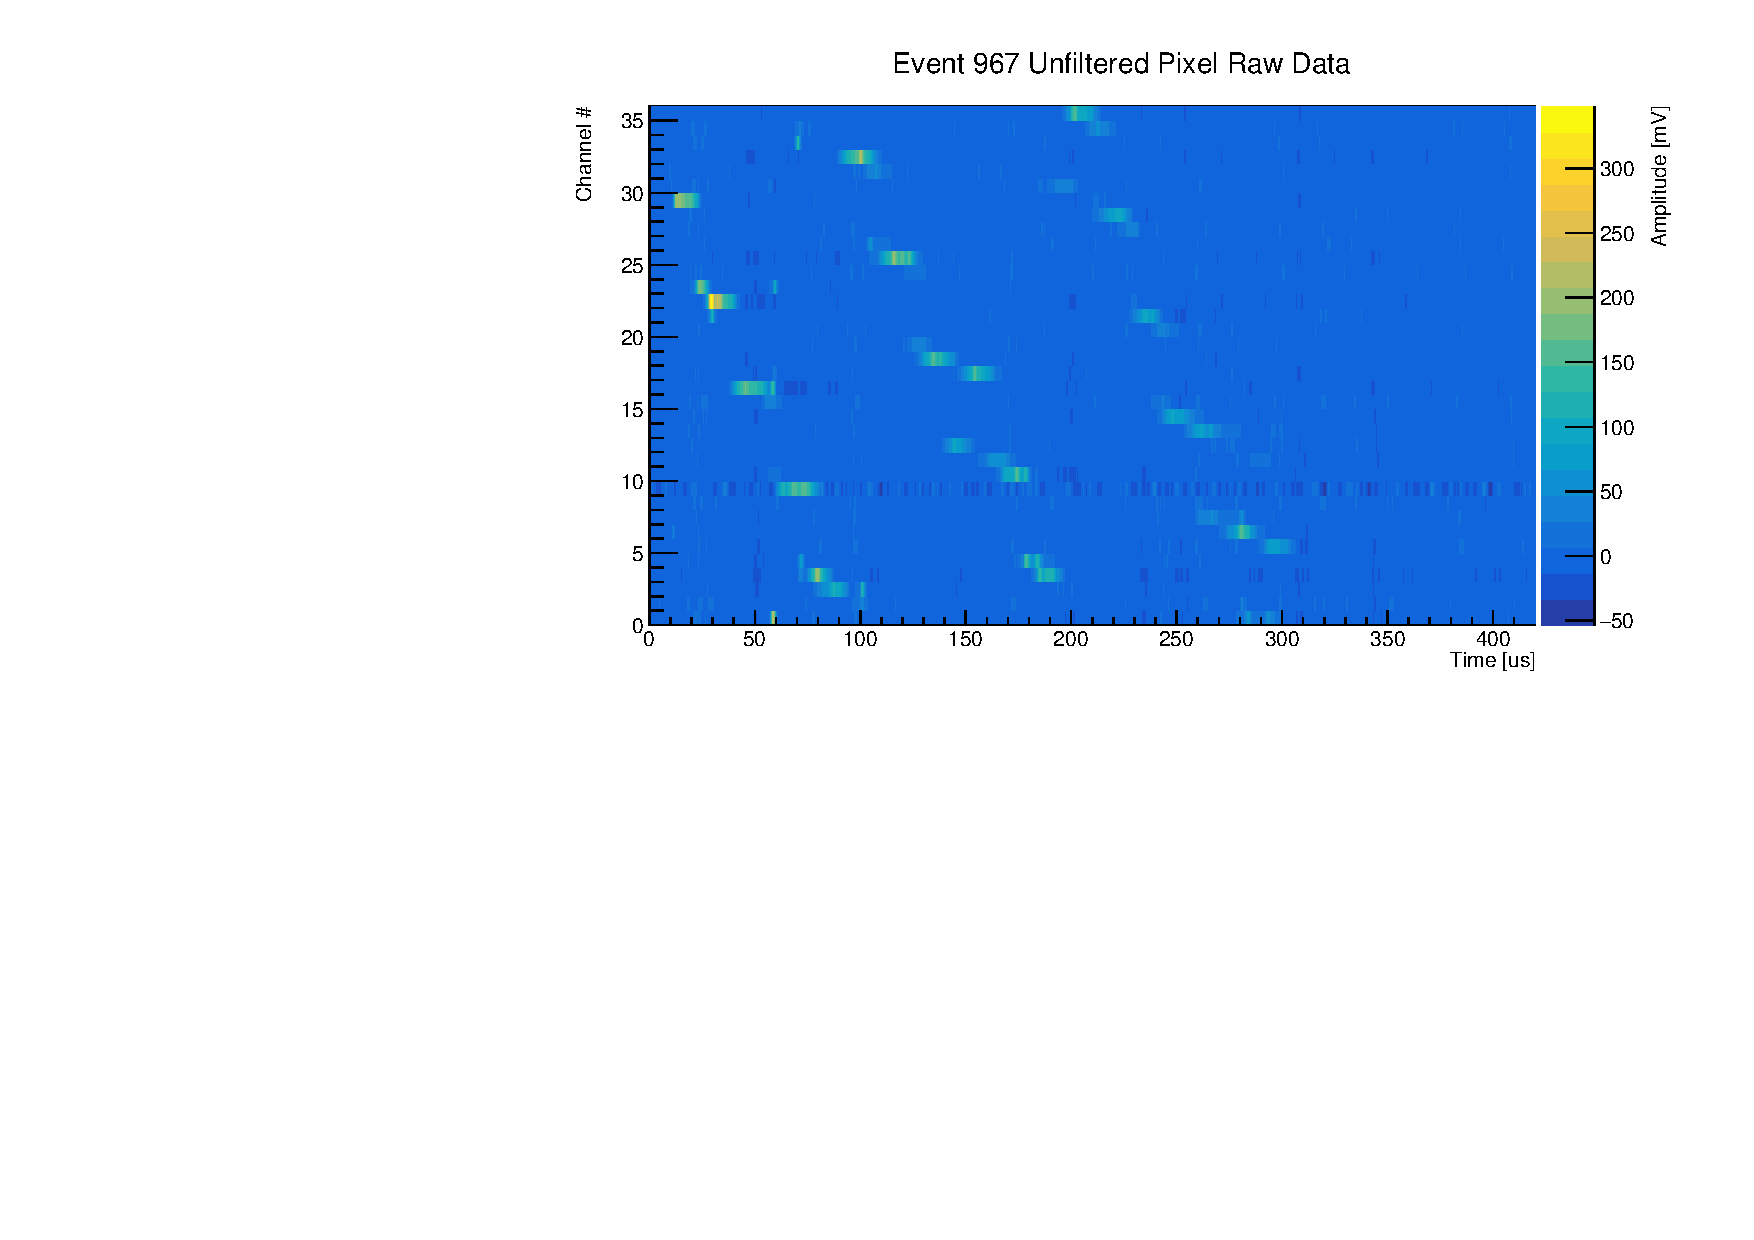
\includegraphics[width=\textwidth]{viper/event967_rawUnfilteredPixel}\\
	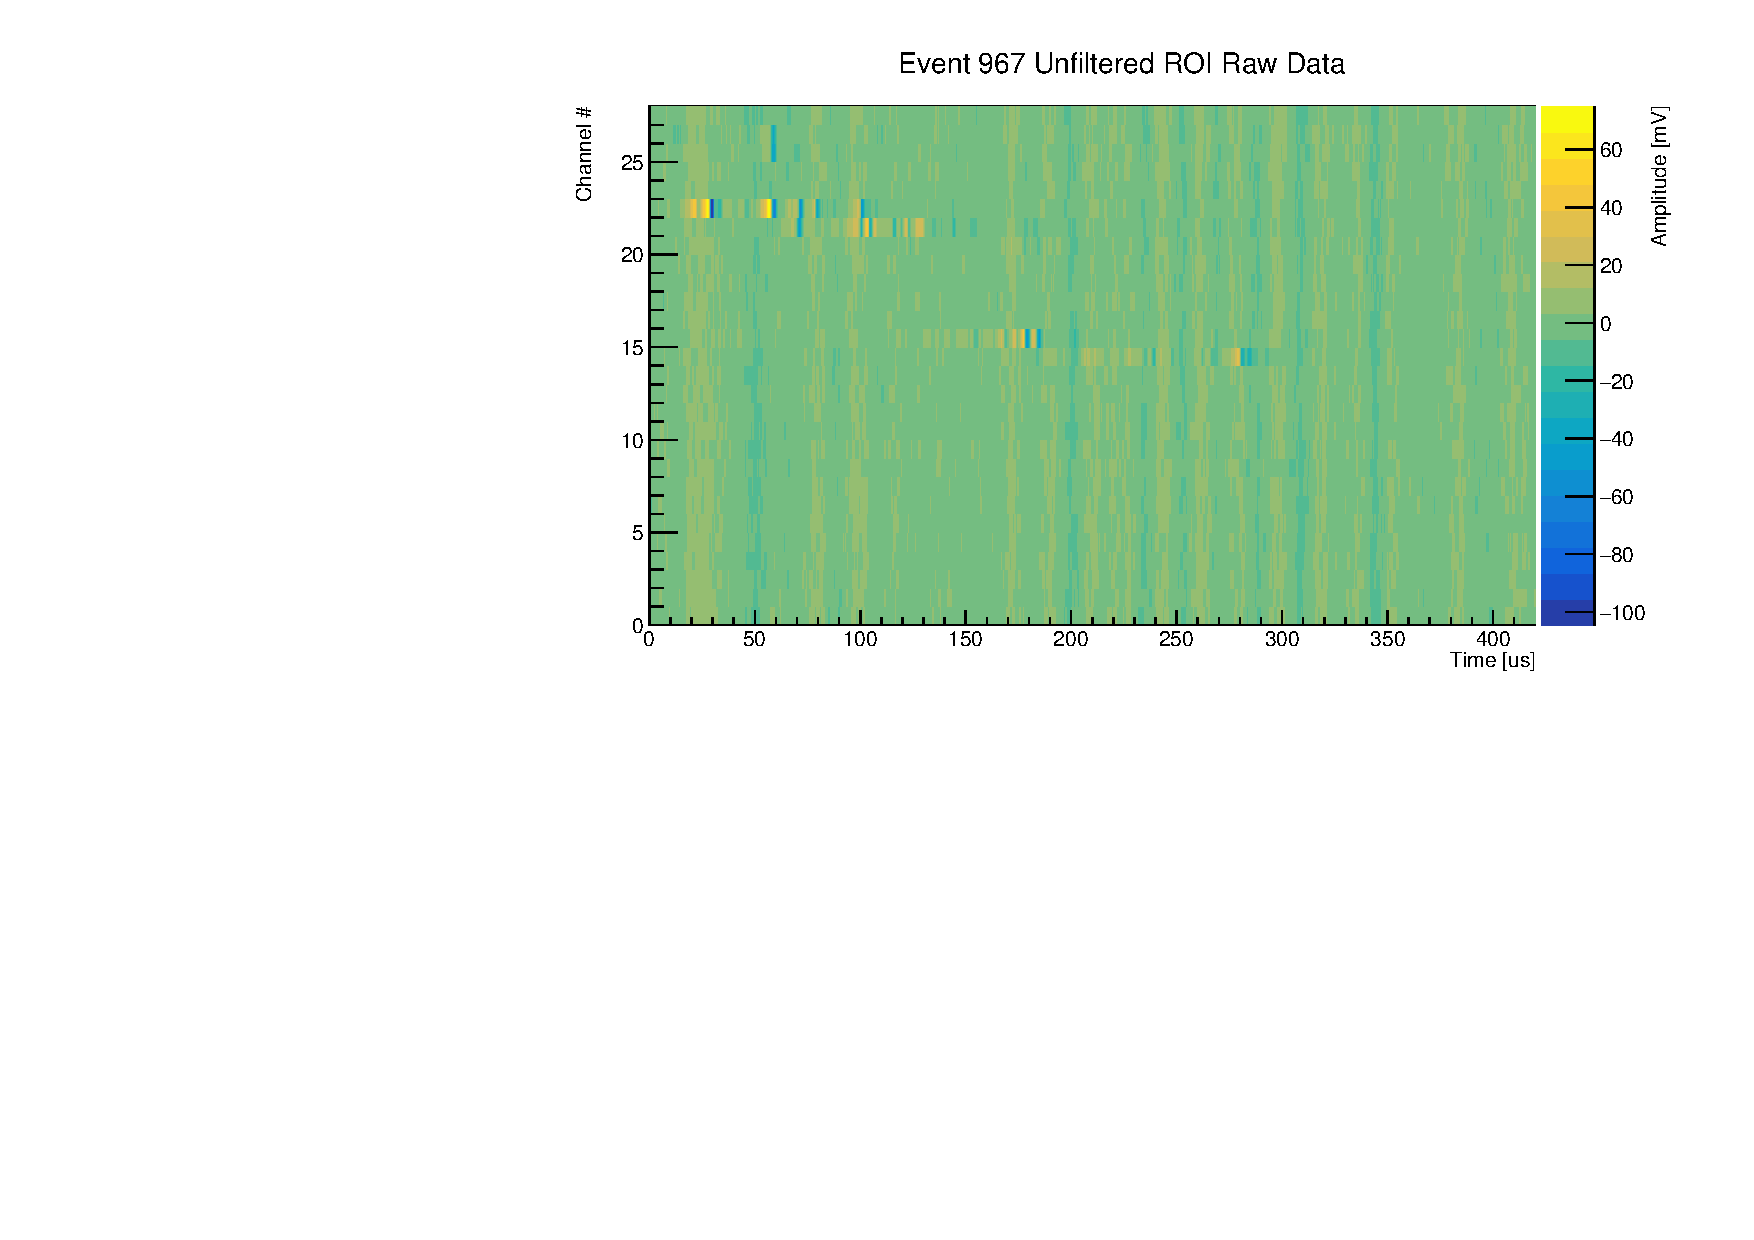
\includegraphics[width=\textwidth]{viper/event967_rawUnfilteredROI}
	\caption[Unfiltered raw data of typical pixel demonstrator event]{%
		Unfiltered raw data of a typical \acrshort{mip} event (the same for Figures~\ref{fig:viper_unfilteredRawData}~through~\ref{fig:viper_kalman}).
		The top plot shows pixel data while the bottom plot shows \acrshort{roi} data.
		Note that the colour scale was adjusted to highlight the charge signals.
		Therefore, most signal peaks are above/below the maximum/minimum of the colour scale.
		The full range of a typical signal can be seen in Figure~\ref{fig:viper_hitFinder}.
	}
	\label{fig:viper_unfilteredRawData}
\end{figure}

To demonstrate \gls{3d} track reconstruction several thousand cosmic ray events were collected with the \AC{} pixel demonstrator described in Section~\ref{sec:ac_viper}, many of which are \glspl{mip}, mostly muons.
The pixelated charge readout was triggered by the cold \gls{sipm} light readout described in Section~\ref{sec:studies_viper-light-ro}.

Official event reconstruction tools were only available for \lartpc{}s read out by wire planes\footnote{\url{http://larsoft.org}}.
Therefore, I developed a new framework from scratch\footnote{\url{https://github.com/70rc/pixy_roimux}}.
The reconstruction procedure comprises five steps: noise filtering, hit finding, hit matching, ambiguity rejection, and track fitting.
These steps are explained in the following and depicted in Figures~\ref{fig:viper_unfilteredRawData} through~\ref{fig:viper_kalman}, all taken from the same \gls{mip} (cosmic muon) event.

\begin{figure}[tbp]
	\centering
	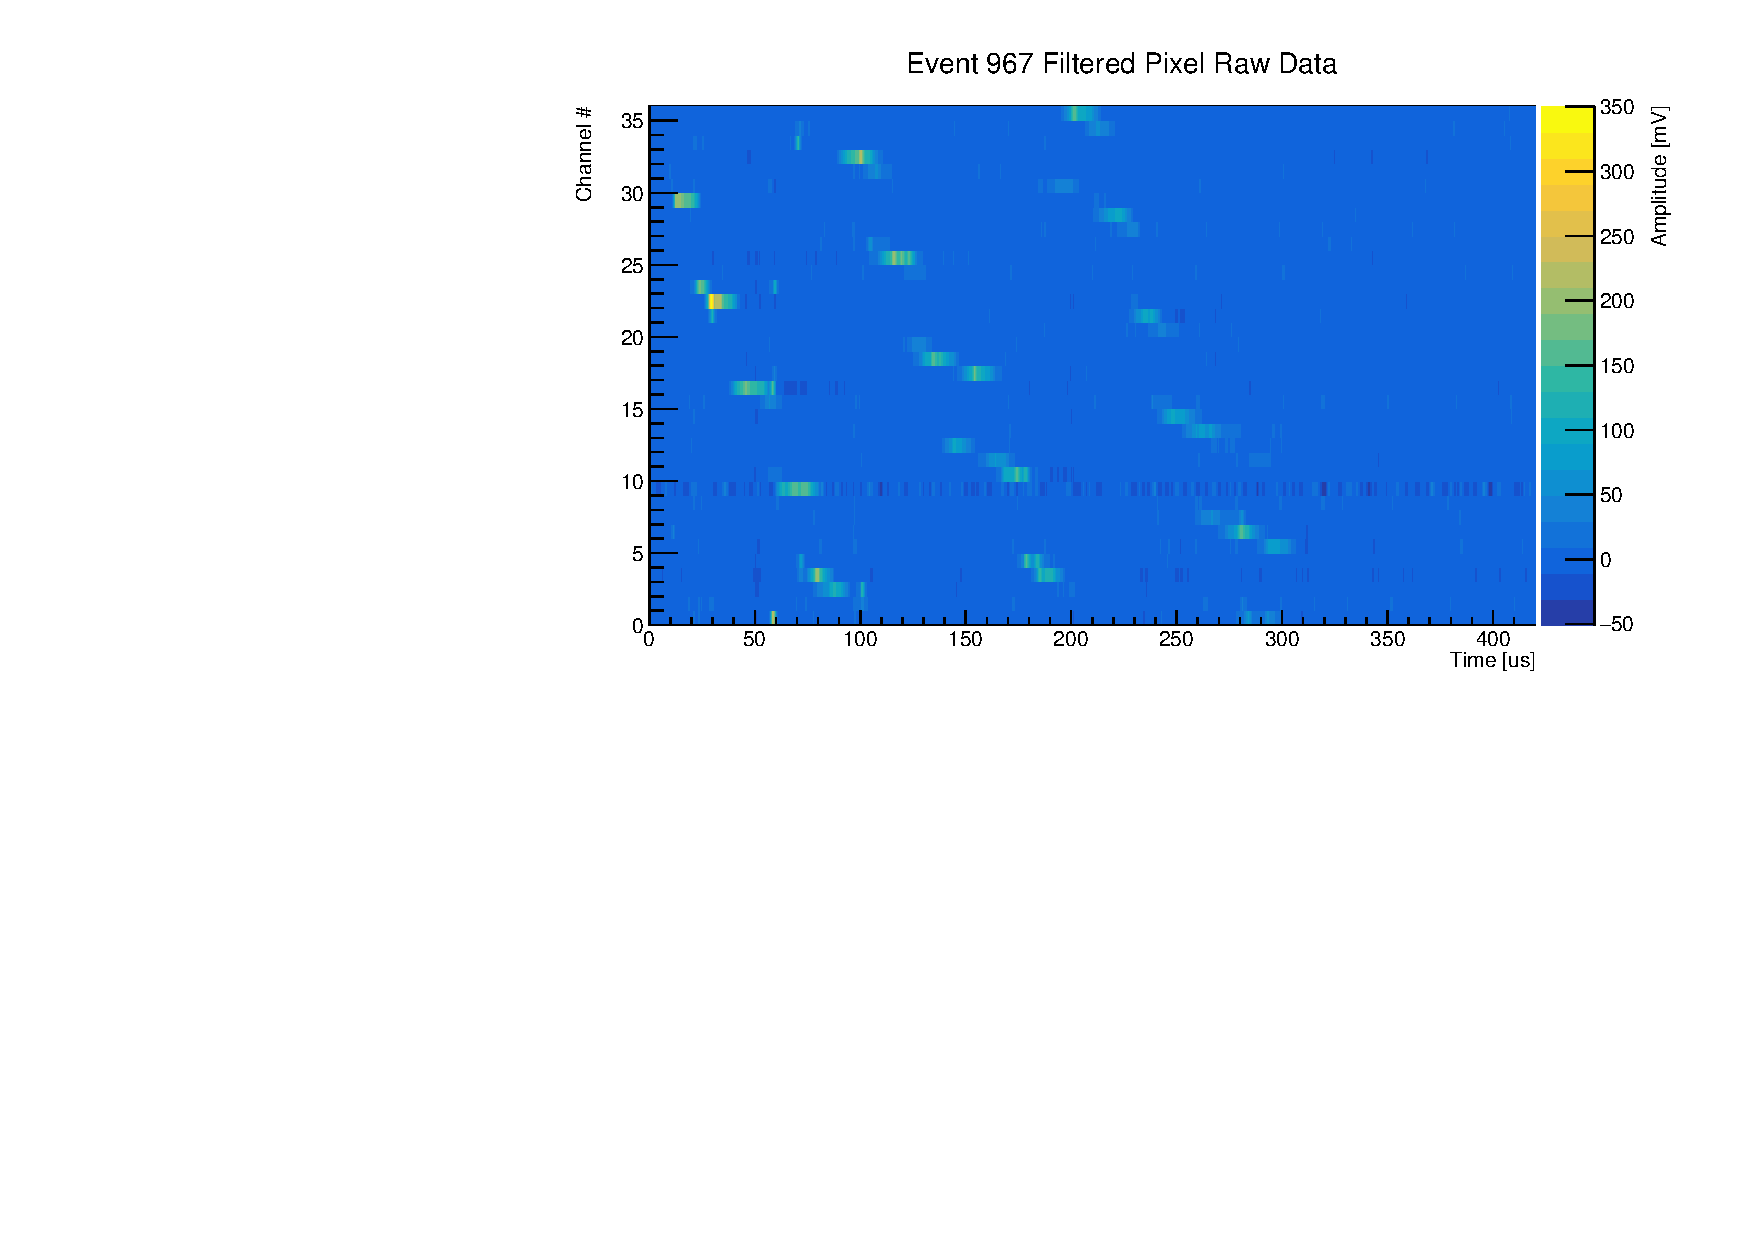
\includegraphics[width=\textwidth]{viper/event967_rawFilteredPixel}\\
	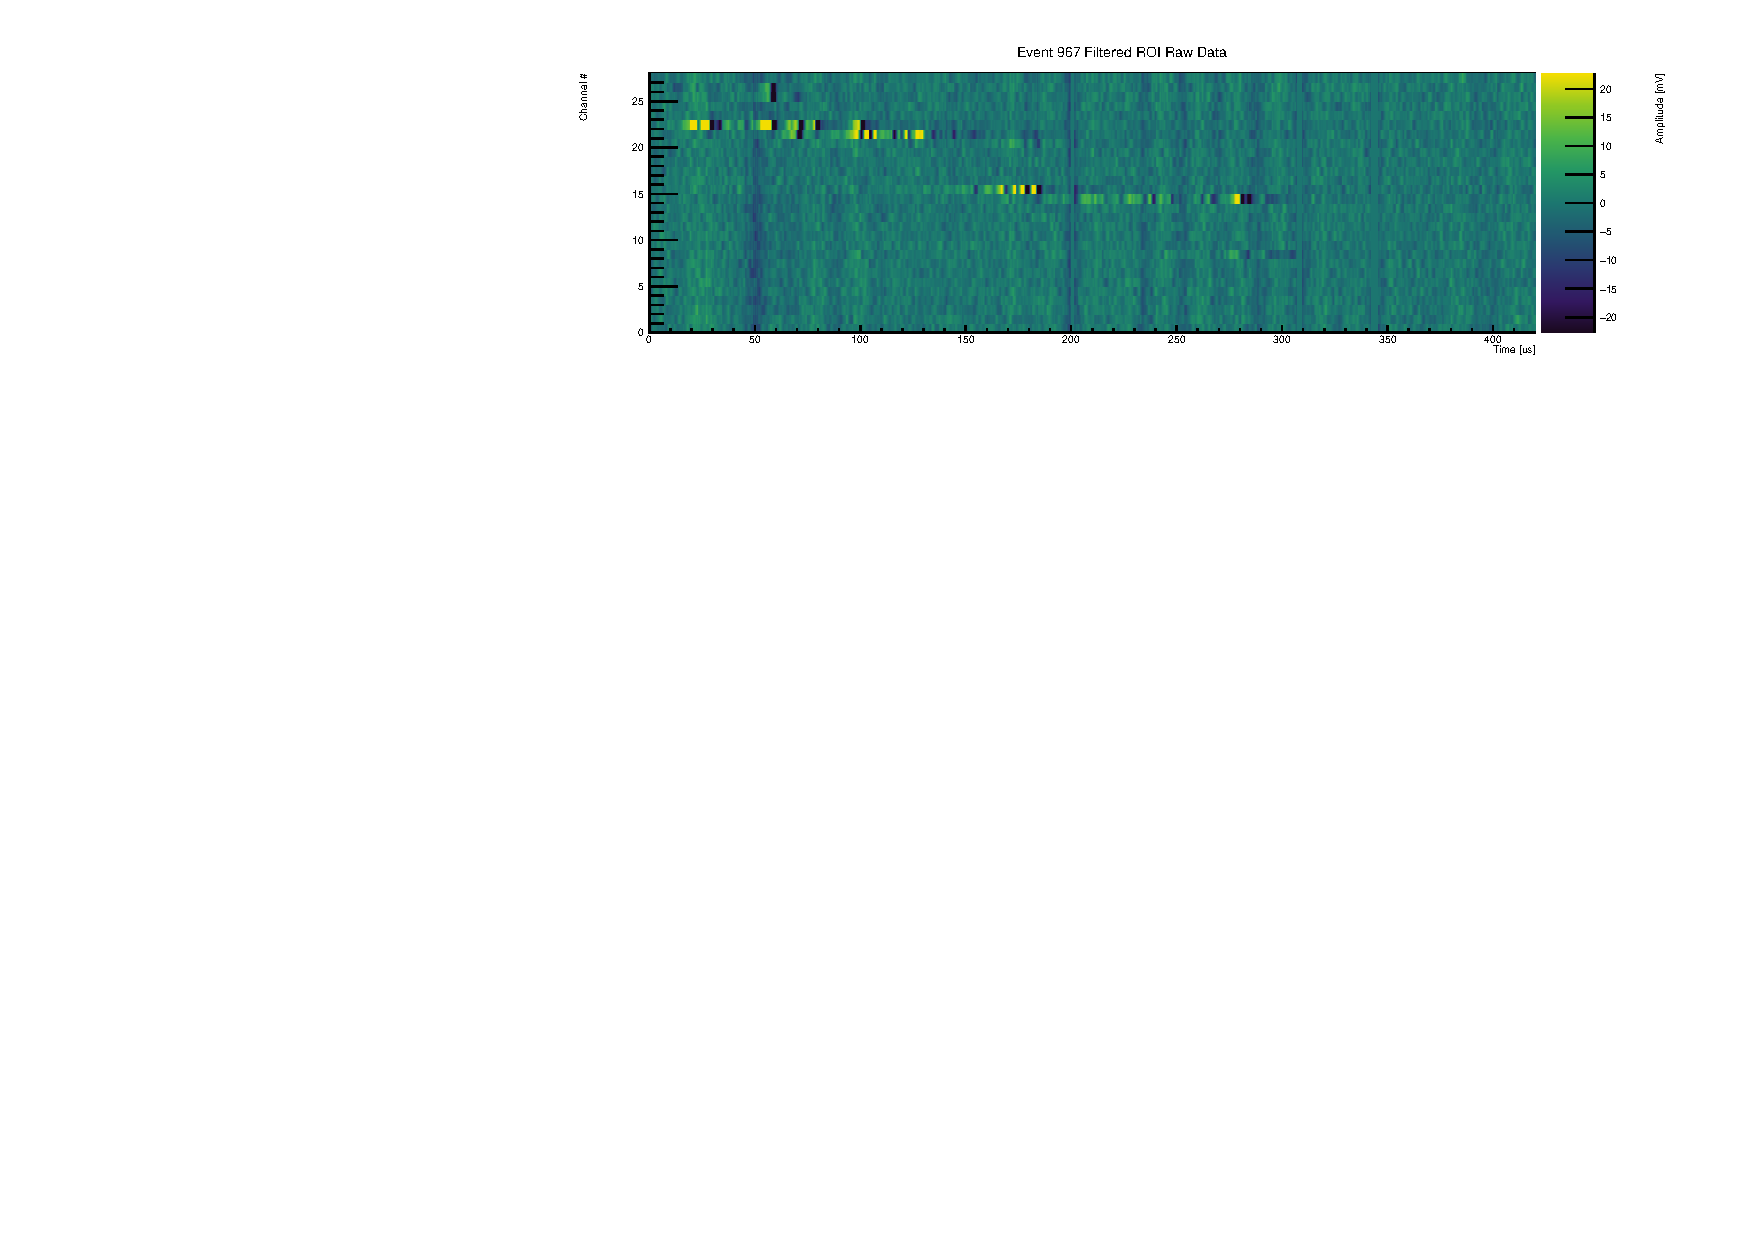
\includegraphics[width=\textwidth]{viper/event967_rawFilteredROI}
	\caption[Filtered data of typical pixel demonstrator event]{%
		Filtered data of a typical \acrshort{mip} event (the same for Figures~\ref{fig:viper_unfilteredRawData}~through~\ref{fig:viper_kalman}).
		The top plot shows pixel data while the bottom plot shows \acrshort{roi} data.
		Note that the colour scale was adjusted to highlight the charge signals.
		Therefore, most signal peaks are above/below the maximum/minimum of the colour scale.
		The full range of a typical signal can be seen in Figure~\ref{fig:viper_hitFinder}.
	}
	\label{fig:viper_filteredRawData}
\end{figure}

In the first step a noise-filtering algorithm is applied to the raw data.
As can be seen from Figure~\ref{fig:viper_unfilteredRawData}, the noise is largely correlated across all the channels.
This common-mode correlation can be exploited by the noise filter algorithm.
The following is done separately for the all pixel and \gls{roi} channels of each event.
Similarly to the \gls{snr} calculation all samples are filled into an amplitude distribution histogram for each channel and subsequently fitted with a Gaussian.
A noise band is defined per channel with its centre equal to the mean of the Gaussian and its width equal to the standard deviation multiplied by a tunable scaling factor.
The amplitudes of all channels within the corresponding noise band are then averaged for each sample.
Finally, this average is subtracted from each channel at the corresponding sample.
This technique was chosen because it effectively suppresses the dominating common-mode noise.
At the same time spurious signals, produced by actual charge collection signals distorting the average, are kept to a minimum by only accepting values within the noise band.
The effectiveness of the filtering can be seen in Figure~\ref{fig:viper_filteredRawData}, which shows the same data as Figure~\ref{fig:viper_unfilteredRawData} post filtering.

\begin{figure}[tbp]
	\centering
	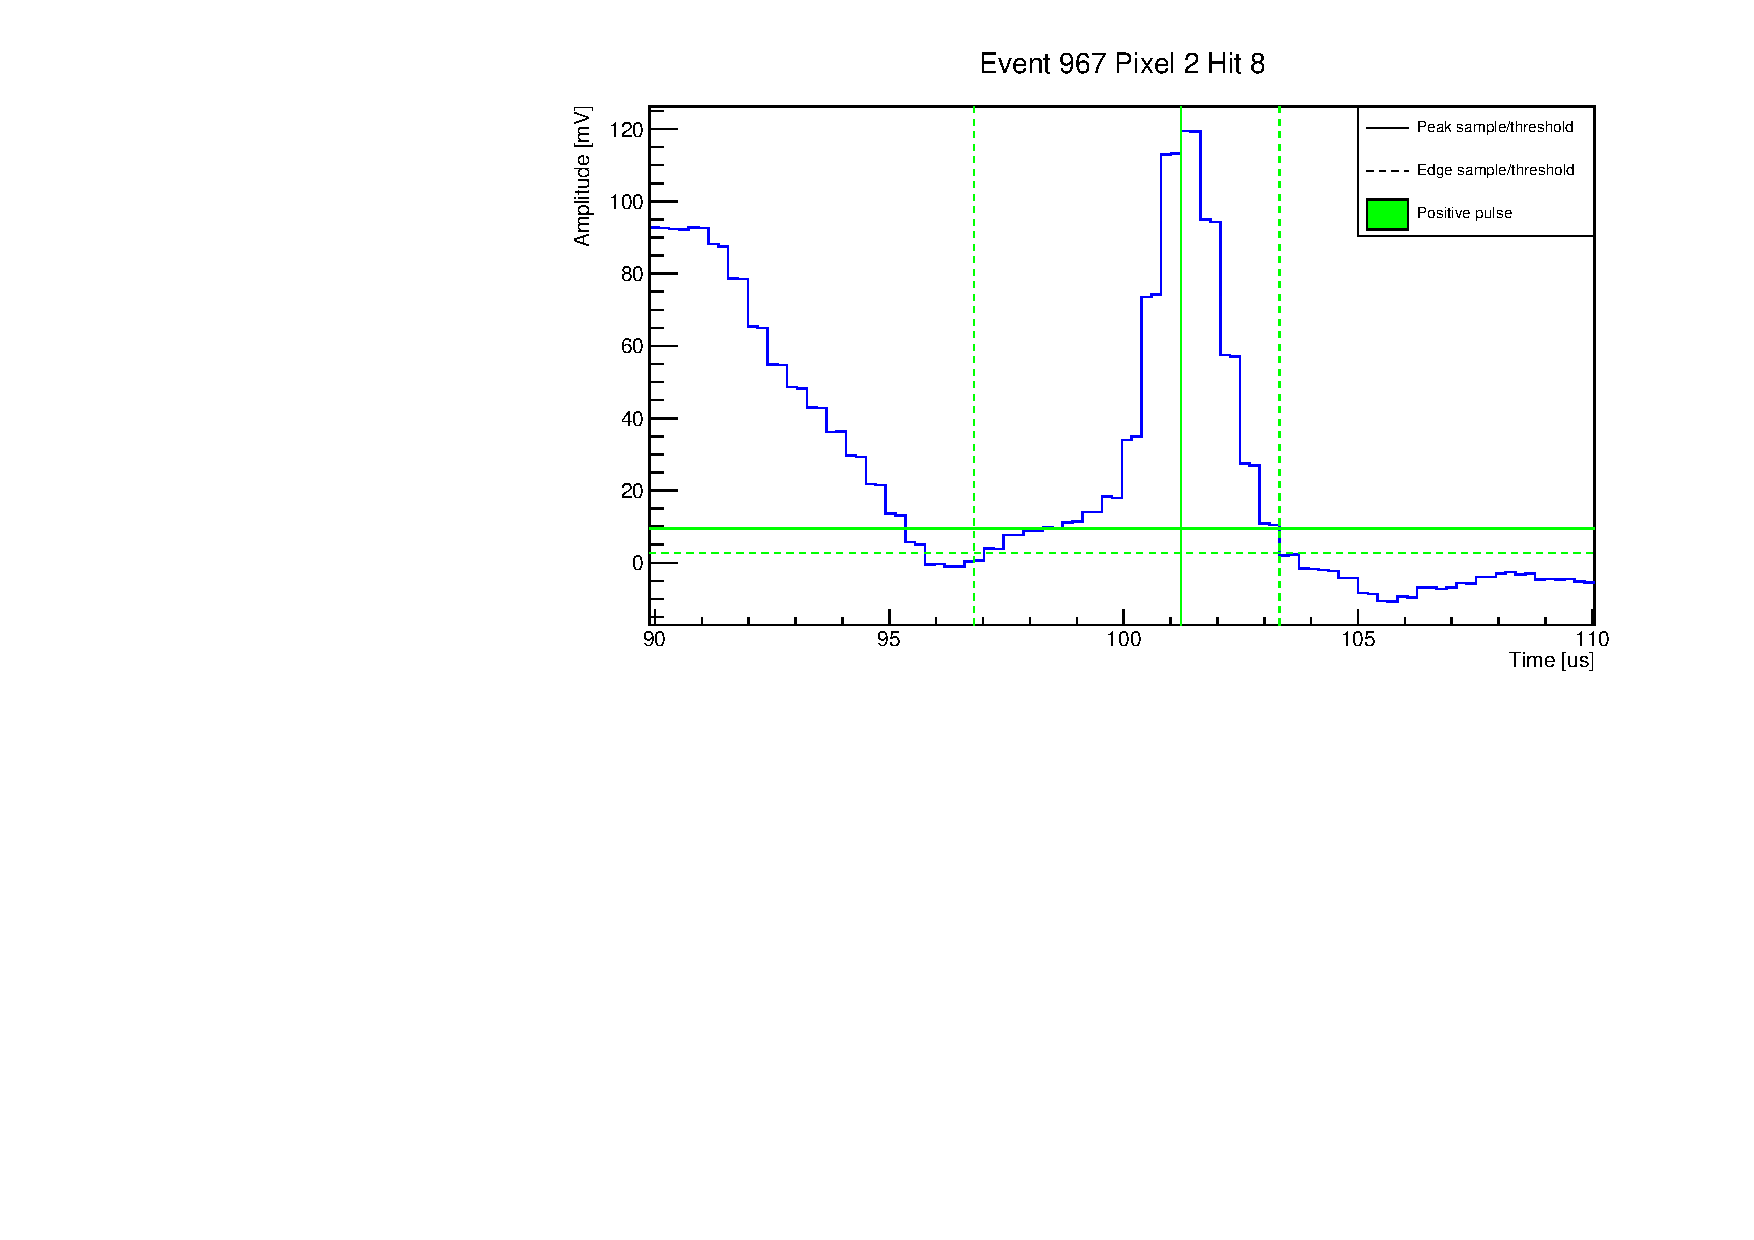
\includegraphics[width=\textwidth, page=1]{viper/event967_pixel2_hit8}\\
	\includegraphics[width=\textwidth, page=3]{viper/event967_pixel2_hit8}
	\caption[Pulse shapes of typical pixel demonstrator event]{%
		Pulse shapes of a single pixel (top) and \acrshort{roi} (bottom) hit of a typical \acrshort{mip} event (the same for Figures~\ref{fig:viper_unfilteredRawData}~through~\ref{fig:viper_kalman}).
		Superimposed are the thresholds of the hit finder algorithm. Horizontal lines represent thresholds: solid is the minimum threshold required to be crossed for a pulse to be detected, and dashed are the thresholds used to detect the pulse edges.
		Vertical lines represent the corresponding detected peak/edge samples.
		Colour indicates a positive (green) or negative (red) pulse, or a zero crossing (yellow).
	}
	\label{fig:viper_hitFinder}
\end{figure}

The second step applies a recursive pulse finding algorithm.
Three types of thresholds are used: peak, edge, and zero-crossing thresholds.
The zero-crossing threshold is equal to the noise mean, as defined above.
Peak and edge thresholds are calculated by adding the noise standard deviation multiplied by a respective scaling factor to the noise mean.
The following is performed for each channel independently.
Noise mean and standard deviation are recalculated from the noise-filtered data.
Using these all thresholds are calculated.
Then, the sample with the highest amplitude is found.
If it is below the peak threshold, the process stops and proceeds to the next channel.
Otherwise, the pulse is scanned in positive and negative directions until it crosses the edge threshold in both directions.
Next, the whole pulse is deleted from the data, and the process starts over with finding the new maximum sample and checking it against the peak threshold.
For stability reasons the peak threshold relative to noise levels is compared against an absolute peak threshold and the higher of the two is applied.
The search is extended to the negative pulse for the bipolar \gls{roi} pulses, using the zero-crossing threshold and respective negative peak and edge thresholds.
The different thresholds employed and samples found by this process are illustrated in Figure~\ref{fig:viper_hitFinder}.

Identified pulses are then combined to \gls{3d} hit candidates by matching pixel pulses to coincident \gls{roi} pulses.
Looking at Figure~\ref{fig:viper_hitFinder}, a pixel and \gls{roi} pulse are matched if their time slices, defined by the vertical dashed lines, overlap.
This matching algorithm minimises the number of missed hits at the price of a rather high number of ambiguous matches.

\begin{figure}[tbp]
	\begin{minipage}{\textwidth}
		\centering
		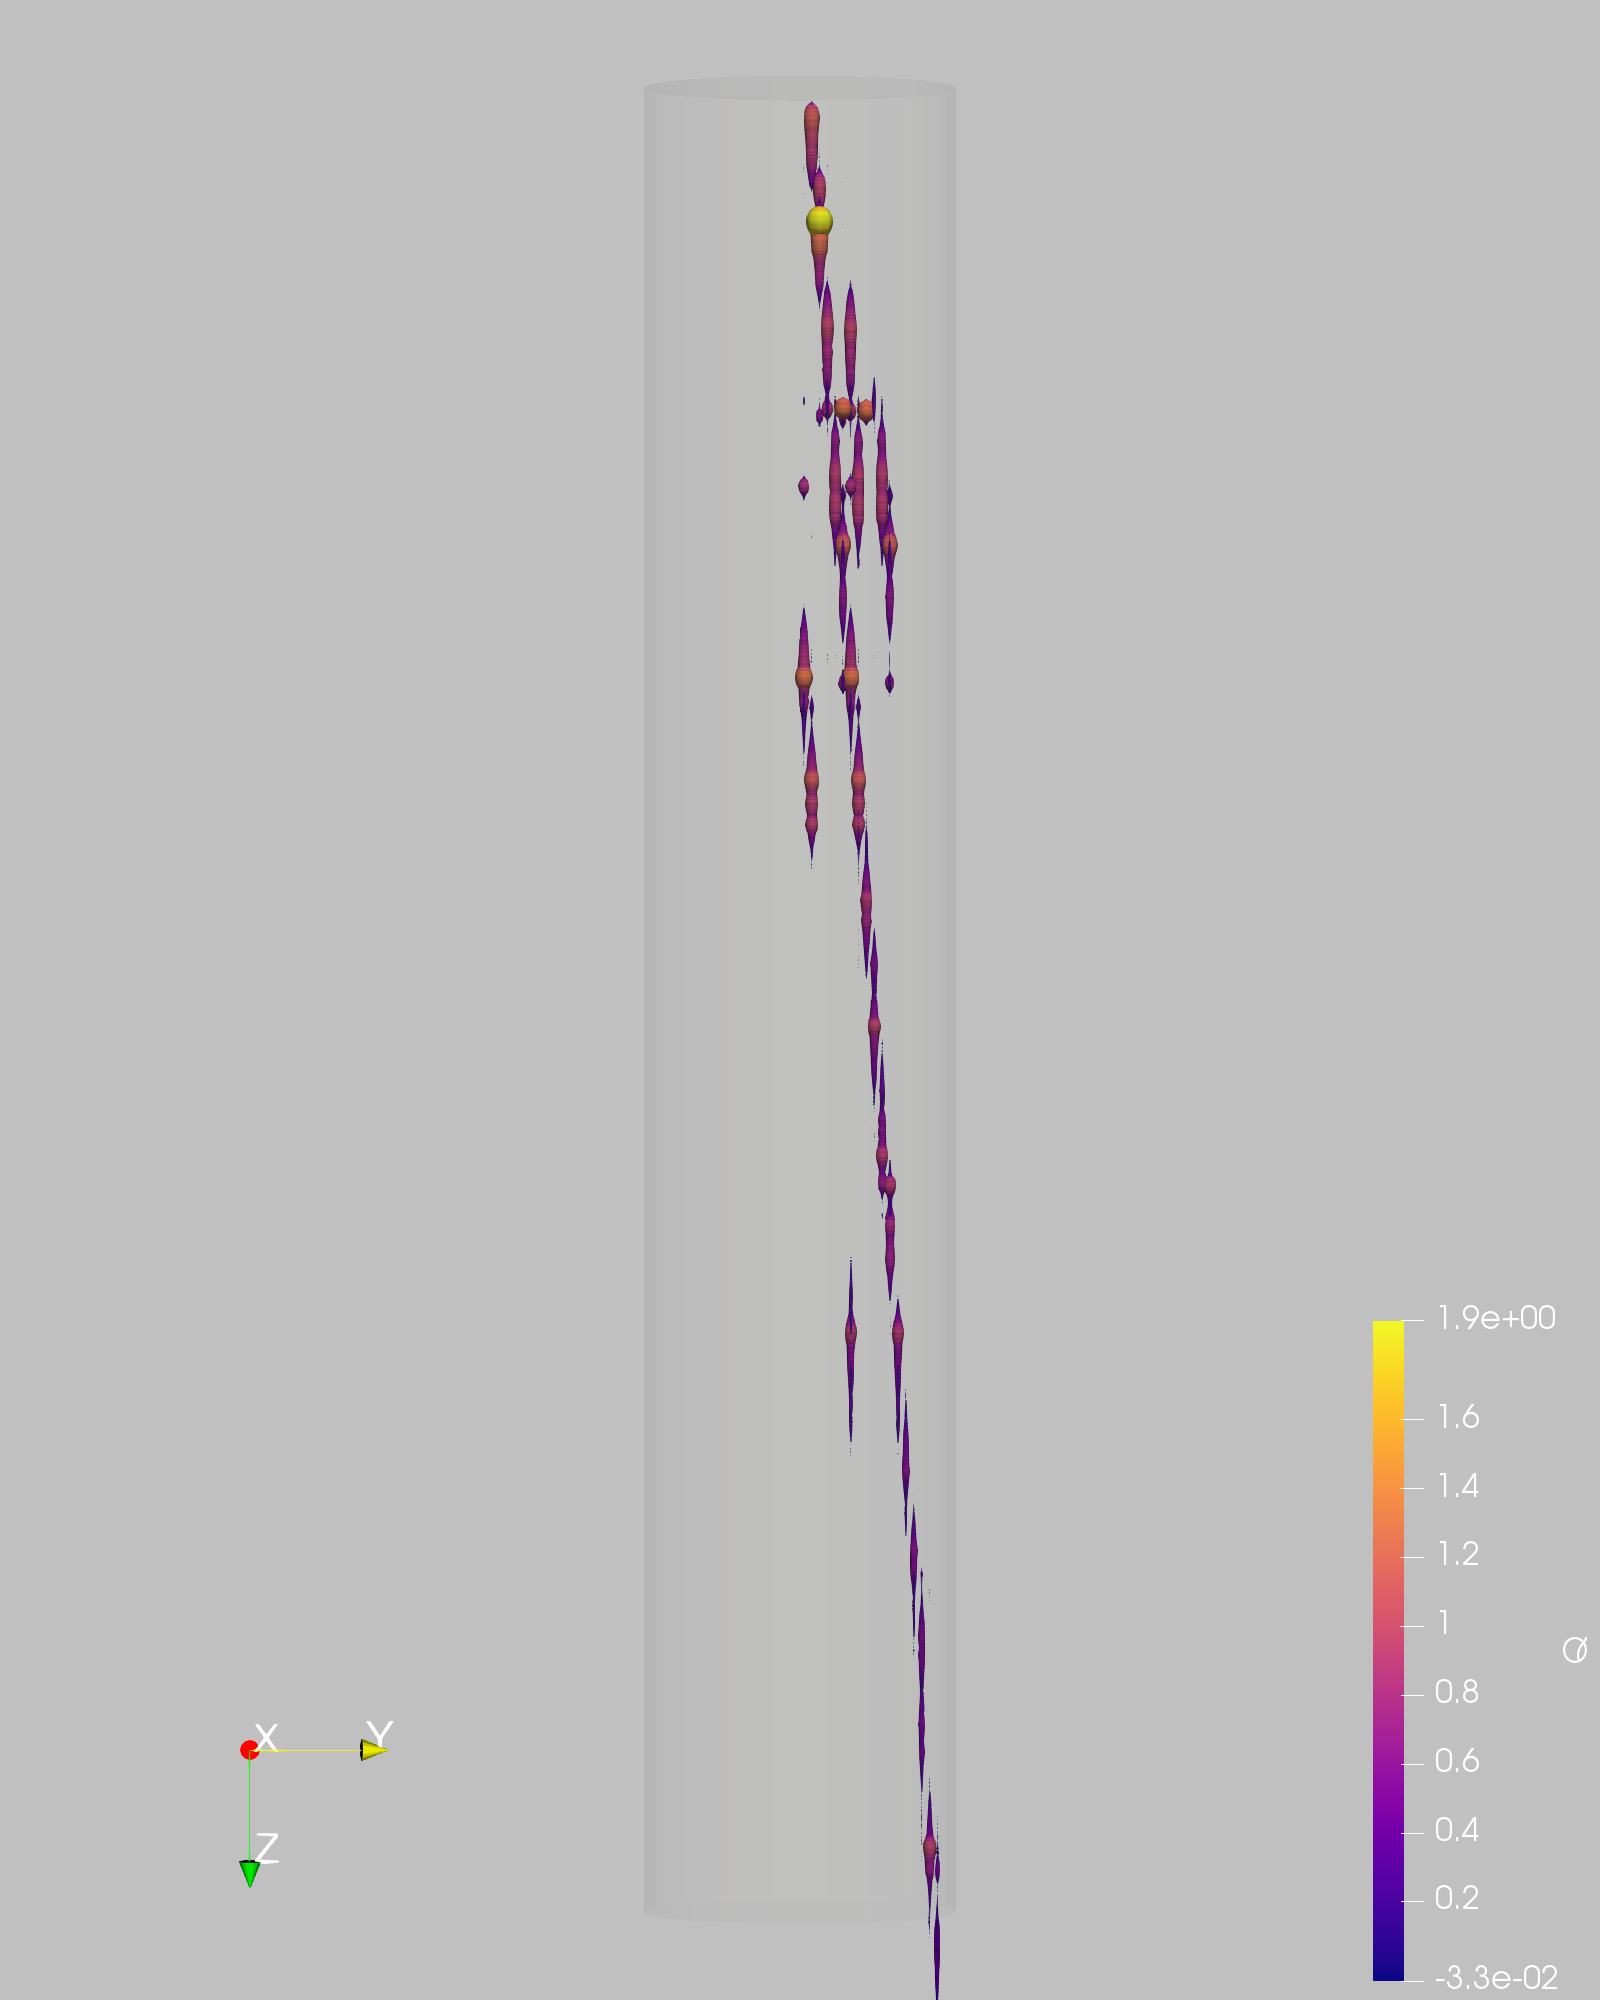
\includegraphics[viewport=600 0 1000 2000, clip, height=\textwidth, angle=90]{viper/event967_pulses_q} \\
		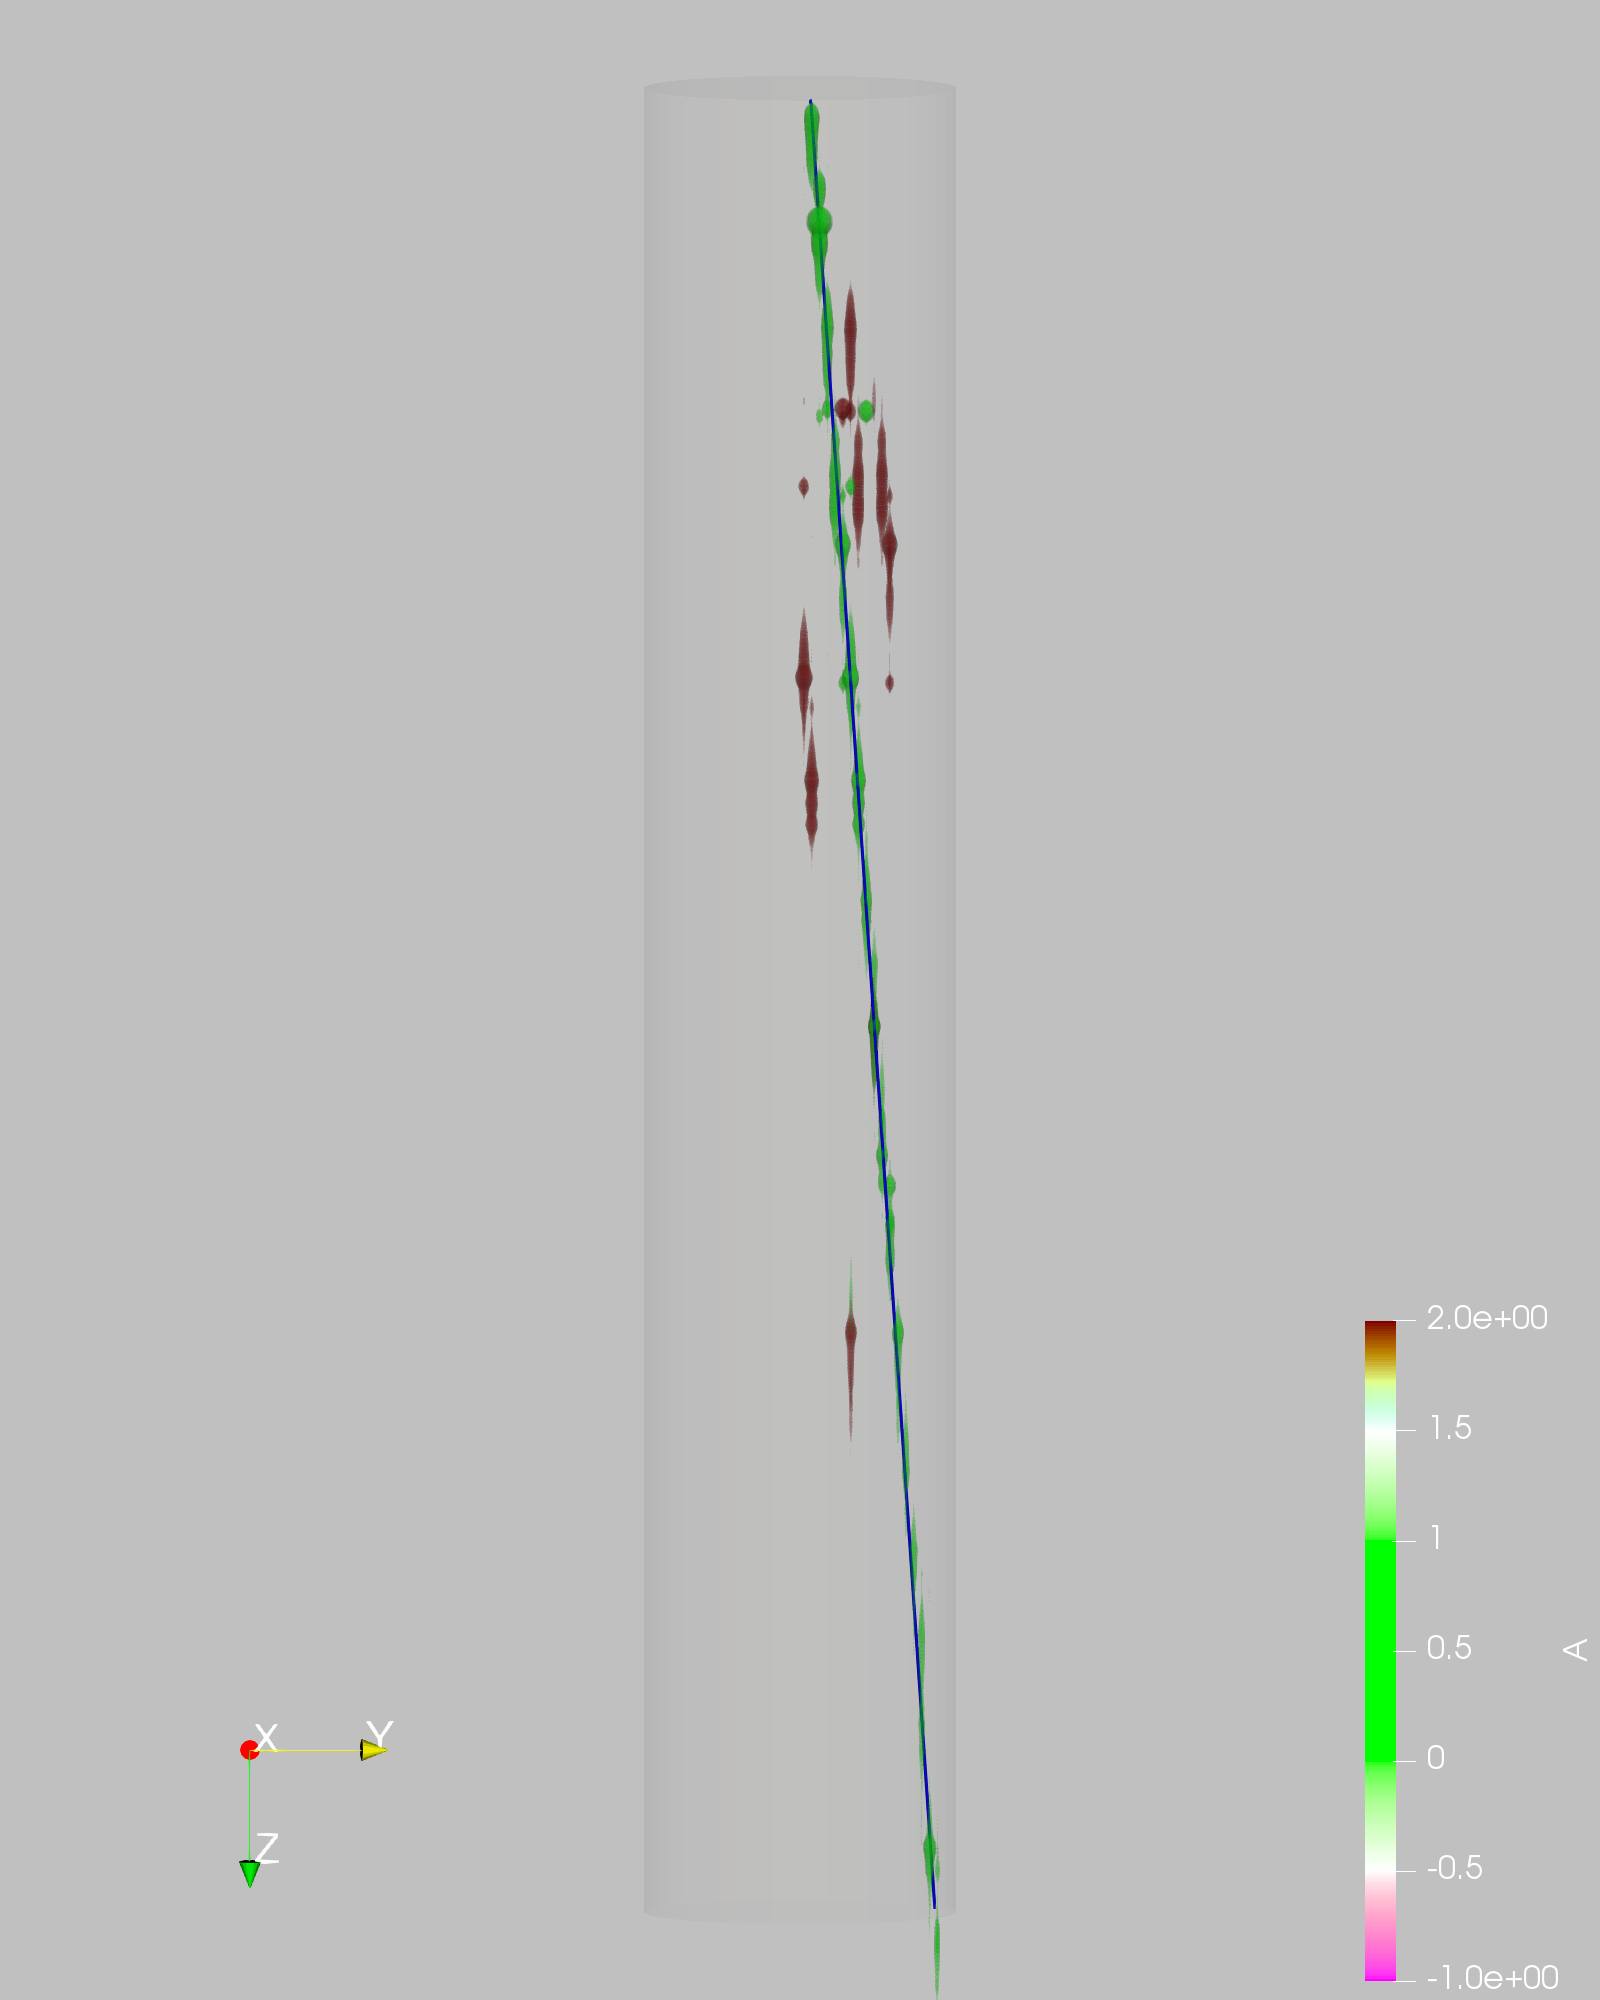
\includegraphics[viewport=600 0 1000 2000, clip, height=\textwidth, angle=90]{viper/event967_pulses_a_pca} \\
		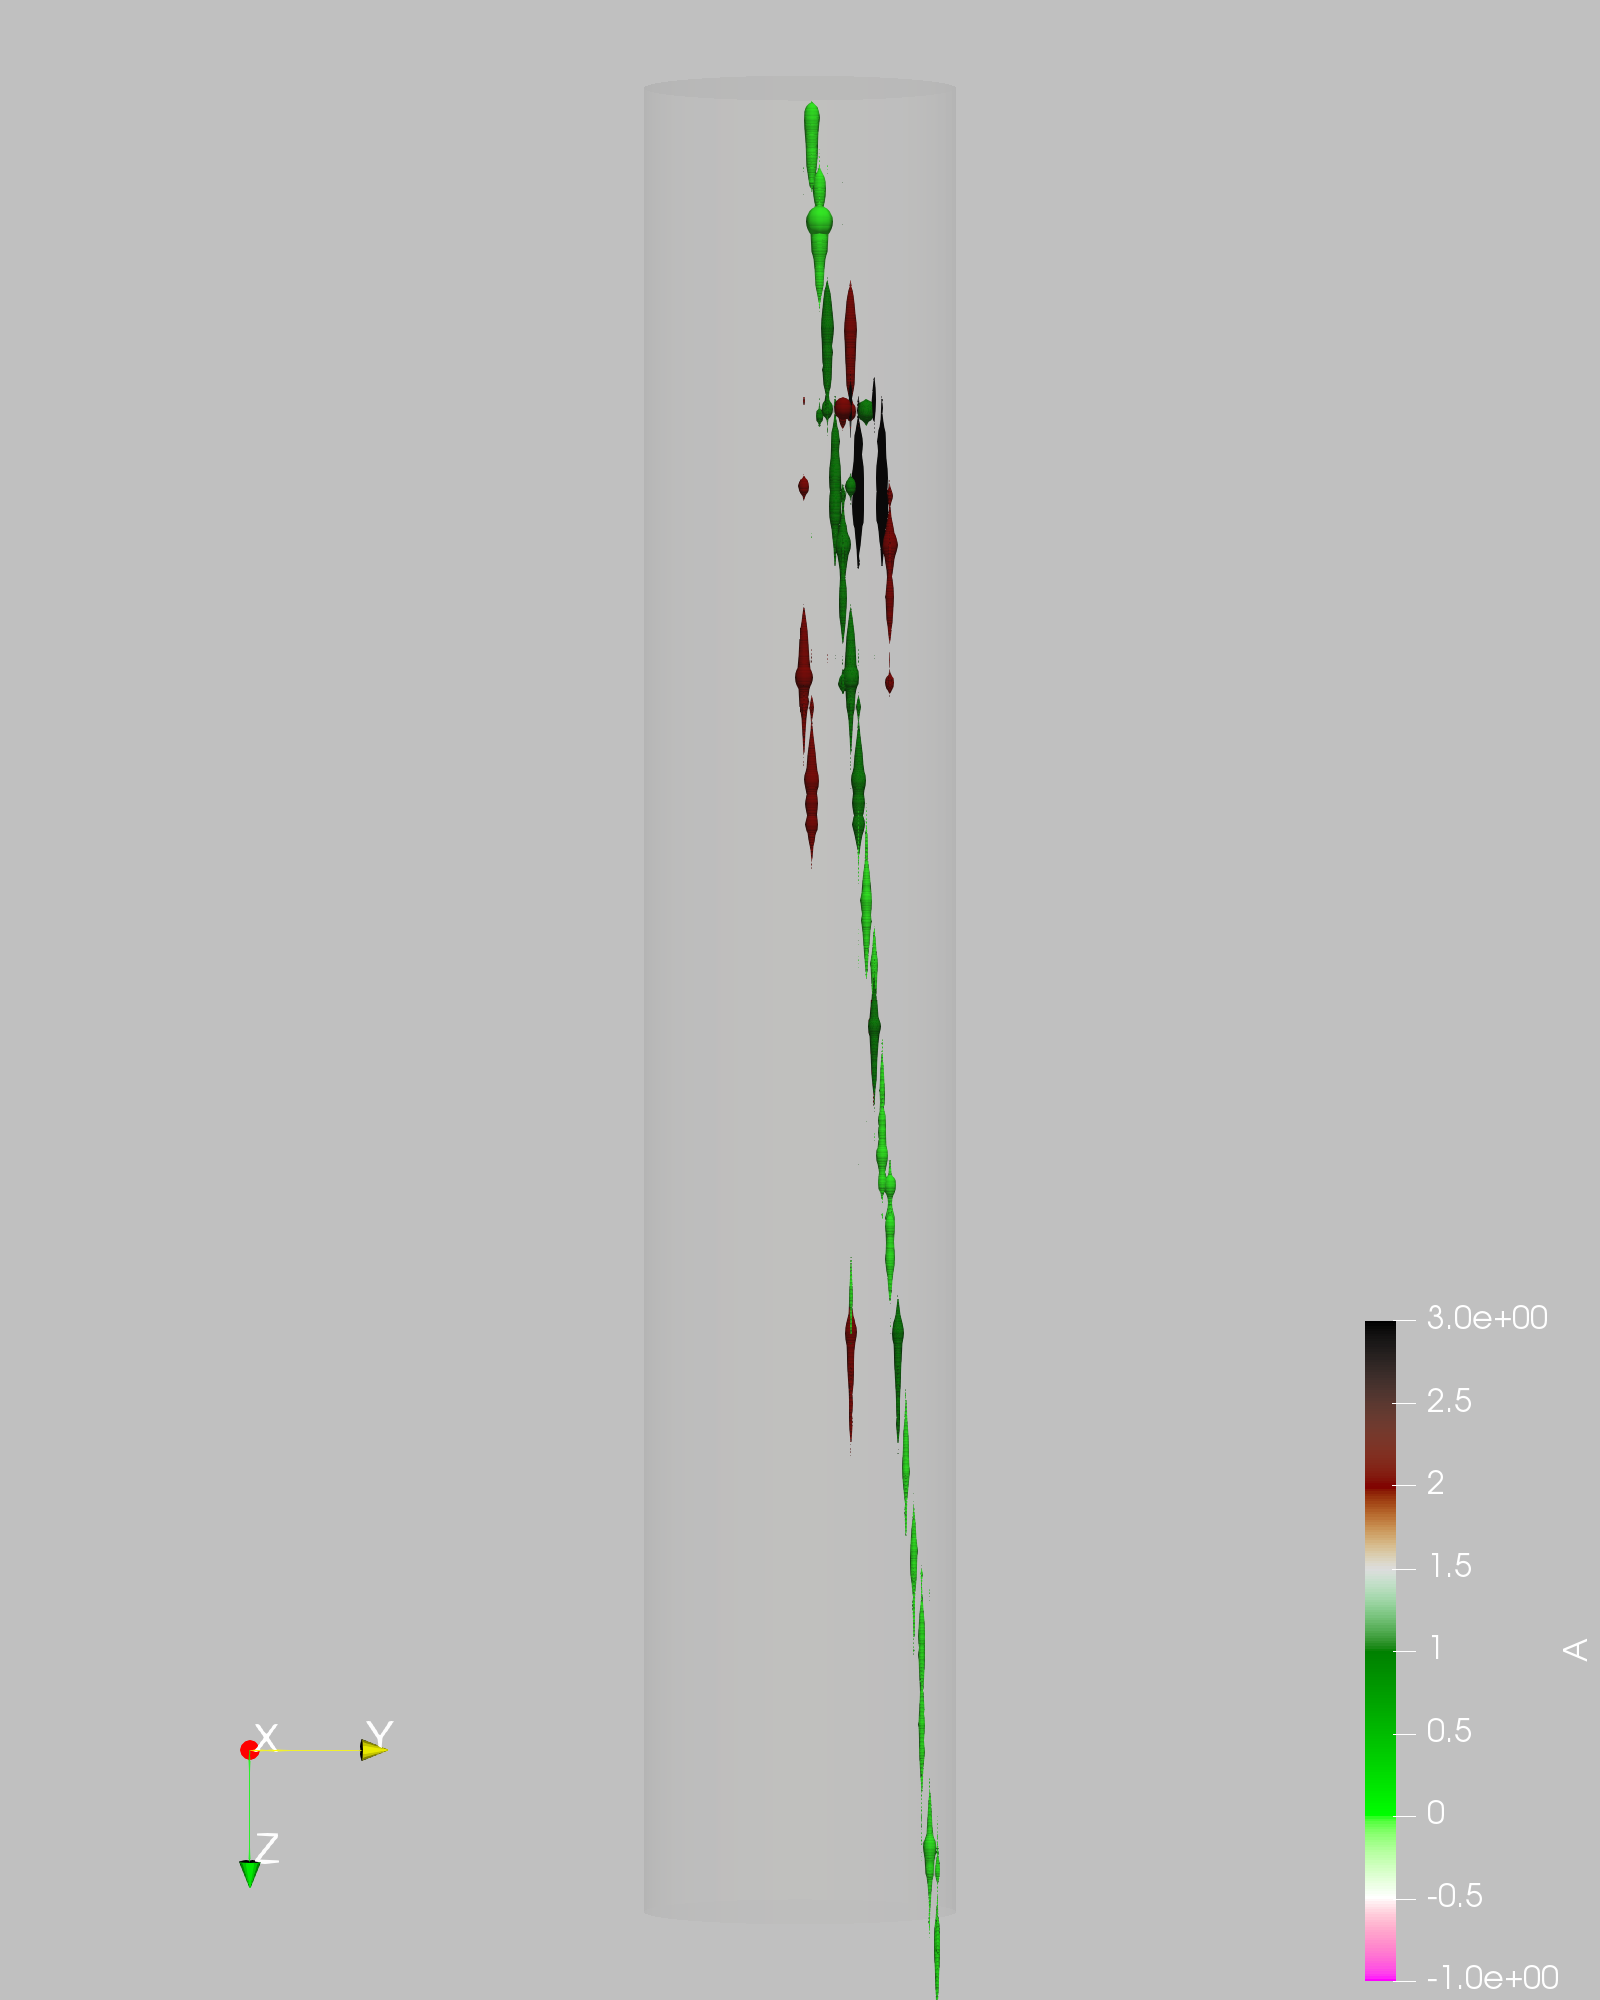
\includegraphics[viewport=600 0 1000 2000, clip, height=\textwidth, angle=90]{viper/event967_pulses_a_det}
		\caption[Reconstructed \glsentryshort{3d} hits of typical pixel demonstrator event]{%
			Reconstructed \acrshort{3d} hit candidates from the hit finder.
			The passing particle is most likely a cosmic \Pgm (the same for Figures~\ref{fig:viper_unfilteredRawData}~through~\ref{fig:viper_kalman}) entering from the left.
			Drift direction is from right to left.
			Pulse shape is encoded as thickness.
			In the top plot colour codes the amount of collected charge.
			The middle plot illustrates the ambiguity resolution employing a \acrshort{pca}.
			Green hit candidates are accepted while dark red ones are rejected.
			This is achieved by selecting the candidate closest to the eigenvector of the point cloud with the largest eigenvalue, represented by the blue line.
			In the bottom plot the degree of ambiguity is colour-coded: Light green are unambiguous hits while dark green are selected candidates of ambiguous hits.
			Dark red through black are rejected candidates of ambiguous hits, where darker colour represents a higher degree of ambiguity.
			As this is quite a clean track with only a few short $\delta$ rays, there are no outliers rejected other than the multiplexing ambiguities.
			Interactive versions of these event displays are available online\footnote{\url{https://70rc.github.io/ac_pix_3d}}.
		}
		\label{fig:viper_pca}
	\end{minipage}
\end{figure}

To resolve the ambiguities a \gls{pca} is applied to the \gls{3d} space points in a fourth step.
This technique is well established and described in literature, e.g.~\cite{pca}.
Therefore, it is only briefly summarised here.
The basic idea is to calculate three orthogonal eigenvectors of the \gls{3d} space point cloud.
A graphic interpretation of these eigenvectors are the three axes of an ellipsoid fitted to the data points.
If the points form a track, one of these eigenvectors will have a much higher eigenvalue than the other two.
This eigenvector is taken as an estimate for the track direction.
Ambiguities can be resolved by selecting the hit candidates closest to the track estimate.
A similar procedure is used to recursively reject outliers, by forming a cylinder around the track estimate with a radius proportional to the second largest eigenvalue.
All hits outside the cylinder are rejected.
The outlier rejection is recursively repeated for an optimal result.
In a later stage of reconstructing more complex events this algorithm can potentially be used to cluster \gls{3d} space points in order to separate multiple tracks.
The \gls{pca} ambiguity rejection is illustrated in Figure~\ref{fig:viper_pca}.

\begin{figure}[tbp]
	\centering
	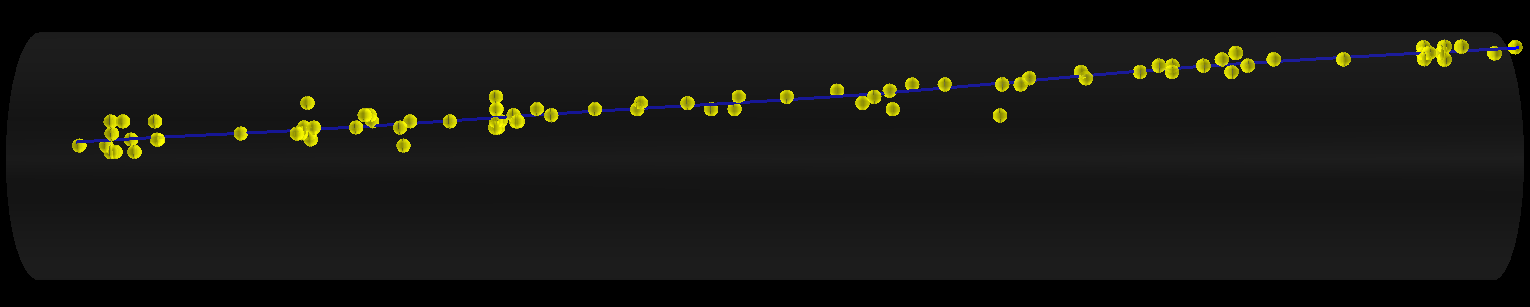
\includegraphics[width=\textwidth]{viper/event967_kalman}
	\caption[Kalman-fitted track of typical pixel demonstrator event]{%
		Track fitted by the Kalman filter.
		The shaded volume represents the \acrshort{tpc}.
		The passing particle is most likely a cosmic \Pgm (the same for Figures~\ref{fig:viper_unfilteredRawData}~through~\ref{fig:viper_kalman}) entering from the left.
		Drift direction is from right to left.
		The yellow points are the input to the Kalman filter, the accepted hits from the \acrshort{pca}.
		Blue is the output, a fitted track taking into account ionisation losses and \acrshort{mcs} in \lar{}.
	}
	\label{fig:viper_kalman}
\end{figure}

The final step consists of a Kalman filter.
For this the well-established \gls{genfit}~\cite{genfit1, genfit2} was used.
Ionisation losses and \gls{mcs} in \lar{} are taken into account.
The particle is assumed to be a minimum-ionising muon with an initial momentum of \SI{260}{\mega\electronvolt\per\clight} in the direction of the track estimate from the \gls{pca}.
A recursive algorithm capable of dealing with outliers was chosen, a so-called \emph{deterministic annealing filter}.
It rejects outliers by assigning successively lower weights to them with each recursion step.
For more details see the respective publications~\cite{genfit1, genfit2}.
The resulting track is shown in Figure~\ref{fig:viper_kalman}.

Technically, the Kalman filter would be capable of fitting the particle momentum or even particle type to the data.
At the time of writing this is not implemented yet.
In particular, the momentum stays roughly at the initial guess of \SI{260}{\mega\electronvolt\per\clight}, assuming a minimum ionising muon in \lar{}.
A potential explanation for this is that the resolution of the detector is too low to estimate momentum from \gls{mcs}.
Another explanation might be the hit finder missing hits due to non-optimal tuning.
Proper tuning of the reconstruction requires a full simulation chain of the detector which is not yet available.
Using data to tune the reconstruction is prone to the introduction of circular biases.
On the other hand, most of the difficulties emerge from the multiplexing ambiguities and their resolution.
While the presented almost full \gls{3d} readout has already reduced the reconstruction complexity compared to a classical wire readout, an ambiguity-free readout will make reconstruction another big step easier by completely eliminating the need to resolve ambiguities.
My results described above triggered the development of the \larpix{} pixel readout electronics at \gls{lbnl}, described in Section~\ref{sec:studies_pixel-electronics}.


\section{\pixlar{}}
\label{sec:ac_pixlar}

\begin{figure}[tbp]
	\centering
	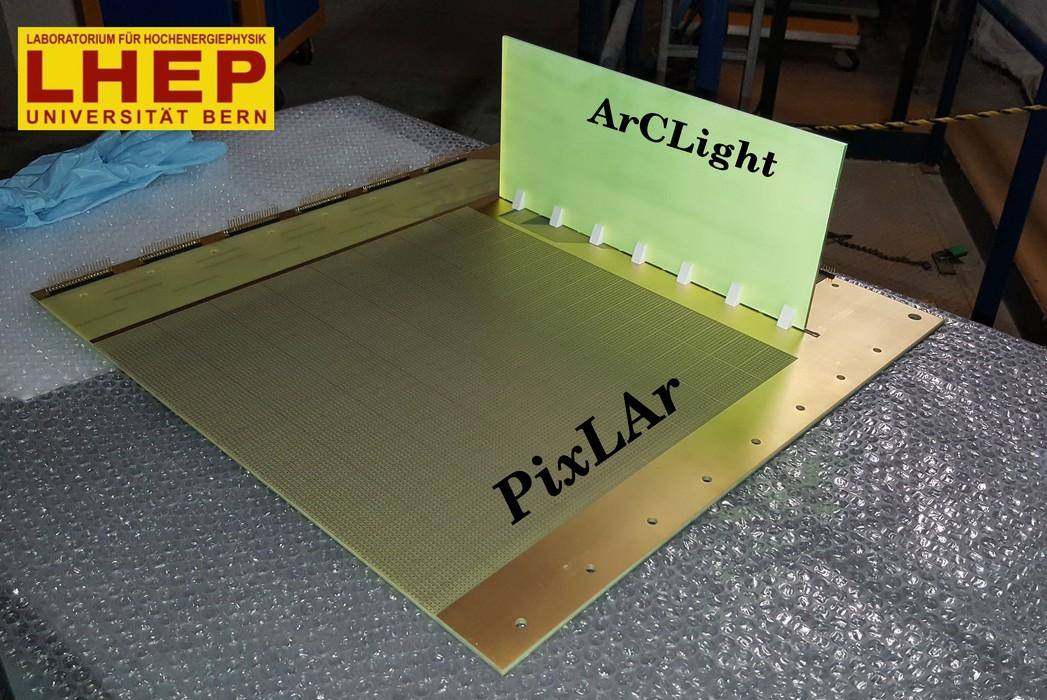
\includegraphics[width=\textwidth]{pixlar/pixlar_arclight}\\
	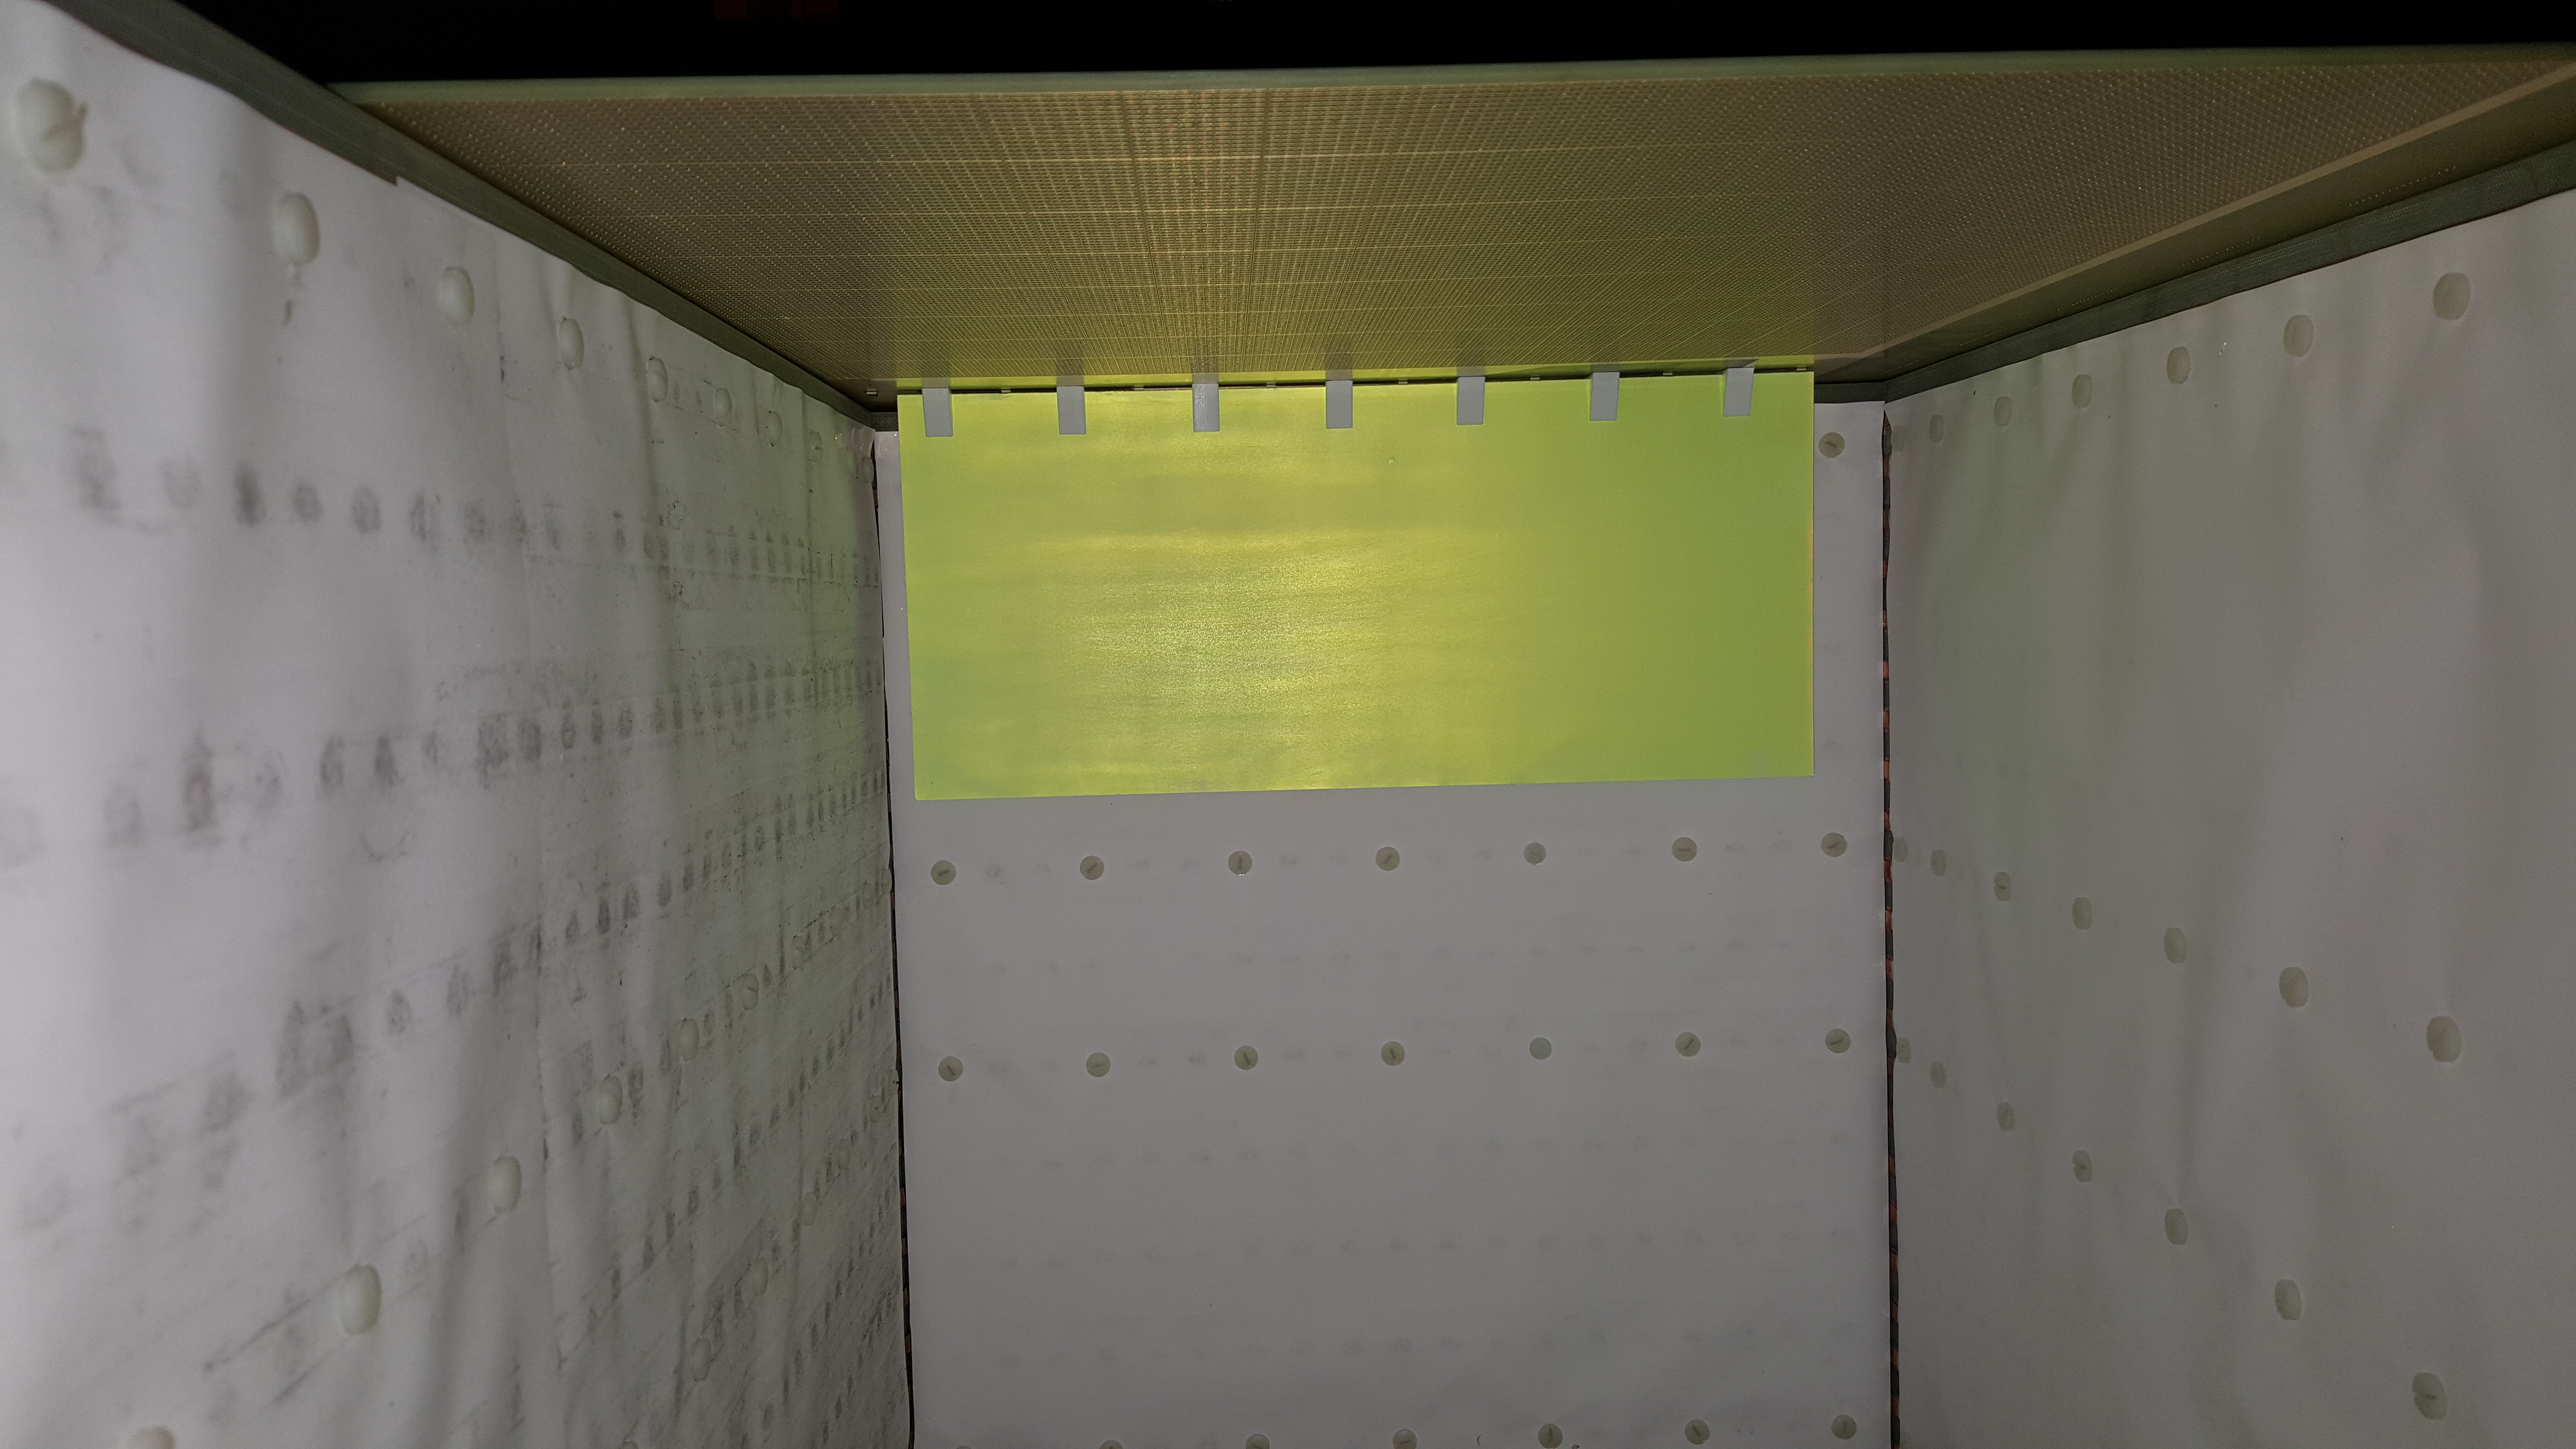
\includegraphics[width=\textwidth]{pixlar/pixlar_arclight_installed}
	\caption[\pixlar{} half plane with attached \glsentryshort{arclight} module]{%
		One of the two \pixlar{} readout half planes with the \acrshort{arclight} module attached.
		The bottom picture shows the inside of the \acrshort{lariat} \acrshort{tpc} with the \pixlar{} \acrshort{arclight} assembly installed.
	}
	\label{fig:pixlar_arclight}
\end{figure}

After my successful test with cosmic muons at \gls{help}, a scaled-up prototype of the pixel readout, employing the same multiplexing scheme, was built for a beam exposure in the \lariat{} experiment~\cite{lariat} at \gls{fail}.
\lariat{} consists of the former \argoneut{}~\cite{argoneut} cryostat and \lartpc{} placed in a test beam.
The tertiary beam line produces mainly pions and protons, as well as electrons, muons, and kaons at a lower rate.
Their momentum spectrum can be tuned from \SIrange{0.2}{2.0}{\giga\electronvolt\per\clight} by means of bending magnets.
\SI{550}{\litre} of \lar{} are contained in a cylindrical cryostat.
It houses a \gls{tpc} with \SI{47}{\centi\metre} drift length and a \SI{40 x 90}{\centi\metre} readout plane parallel to the beam direction, resulting in an active volume of \SI{170}{\litre}.
For the pixel test, called \pixlar{}, the original wire planes were replaced by a \num{120 x 240} pixel readout.
At \SI{3}{\milli\metre} pitch this gives an instrumented area of \SI{36 x 72}{\centi\metre}.
The readout plane had to be split into two mirror-symmetric, electrically independent half planes due to constraints from the \gls{pcb} manufacturer.
Each \num{120 x 120} pixel half plane is divided into \num{8 x 15} \glspl{roi} of \num{15 x 8} pixels each.
The \glspl{roi} are oriented with their longer dimension parallel to the beam direction to reduce the multiplexing ambiguities.
One of the noise mitigation measures implemented for the \gls{help} pixel demonstrator was to use the same differential warm signal path as used by \lariat{}.
Therefore, the charge readout electronics used in \pixlar{} are quite similar to the \AT{} chain described in Section~\ref{sec:studies_at-ro} after the upgrades.
To trigger on scintillation light one end of the \gls{tpc} is equipped with a \SI{43 x 15}{\centi\metre} \AL{} module (see Section~\ref{sec:studies_arclight}) while the other end features an \gls{arapuca}~\cite{arapuca} detector for comparison.
Figure~\ref{fig:pixlar_arclight} shows one of the readout half planes with the \AL{} module attached.

\begin{figure}[tbp]
	\centering
	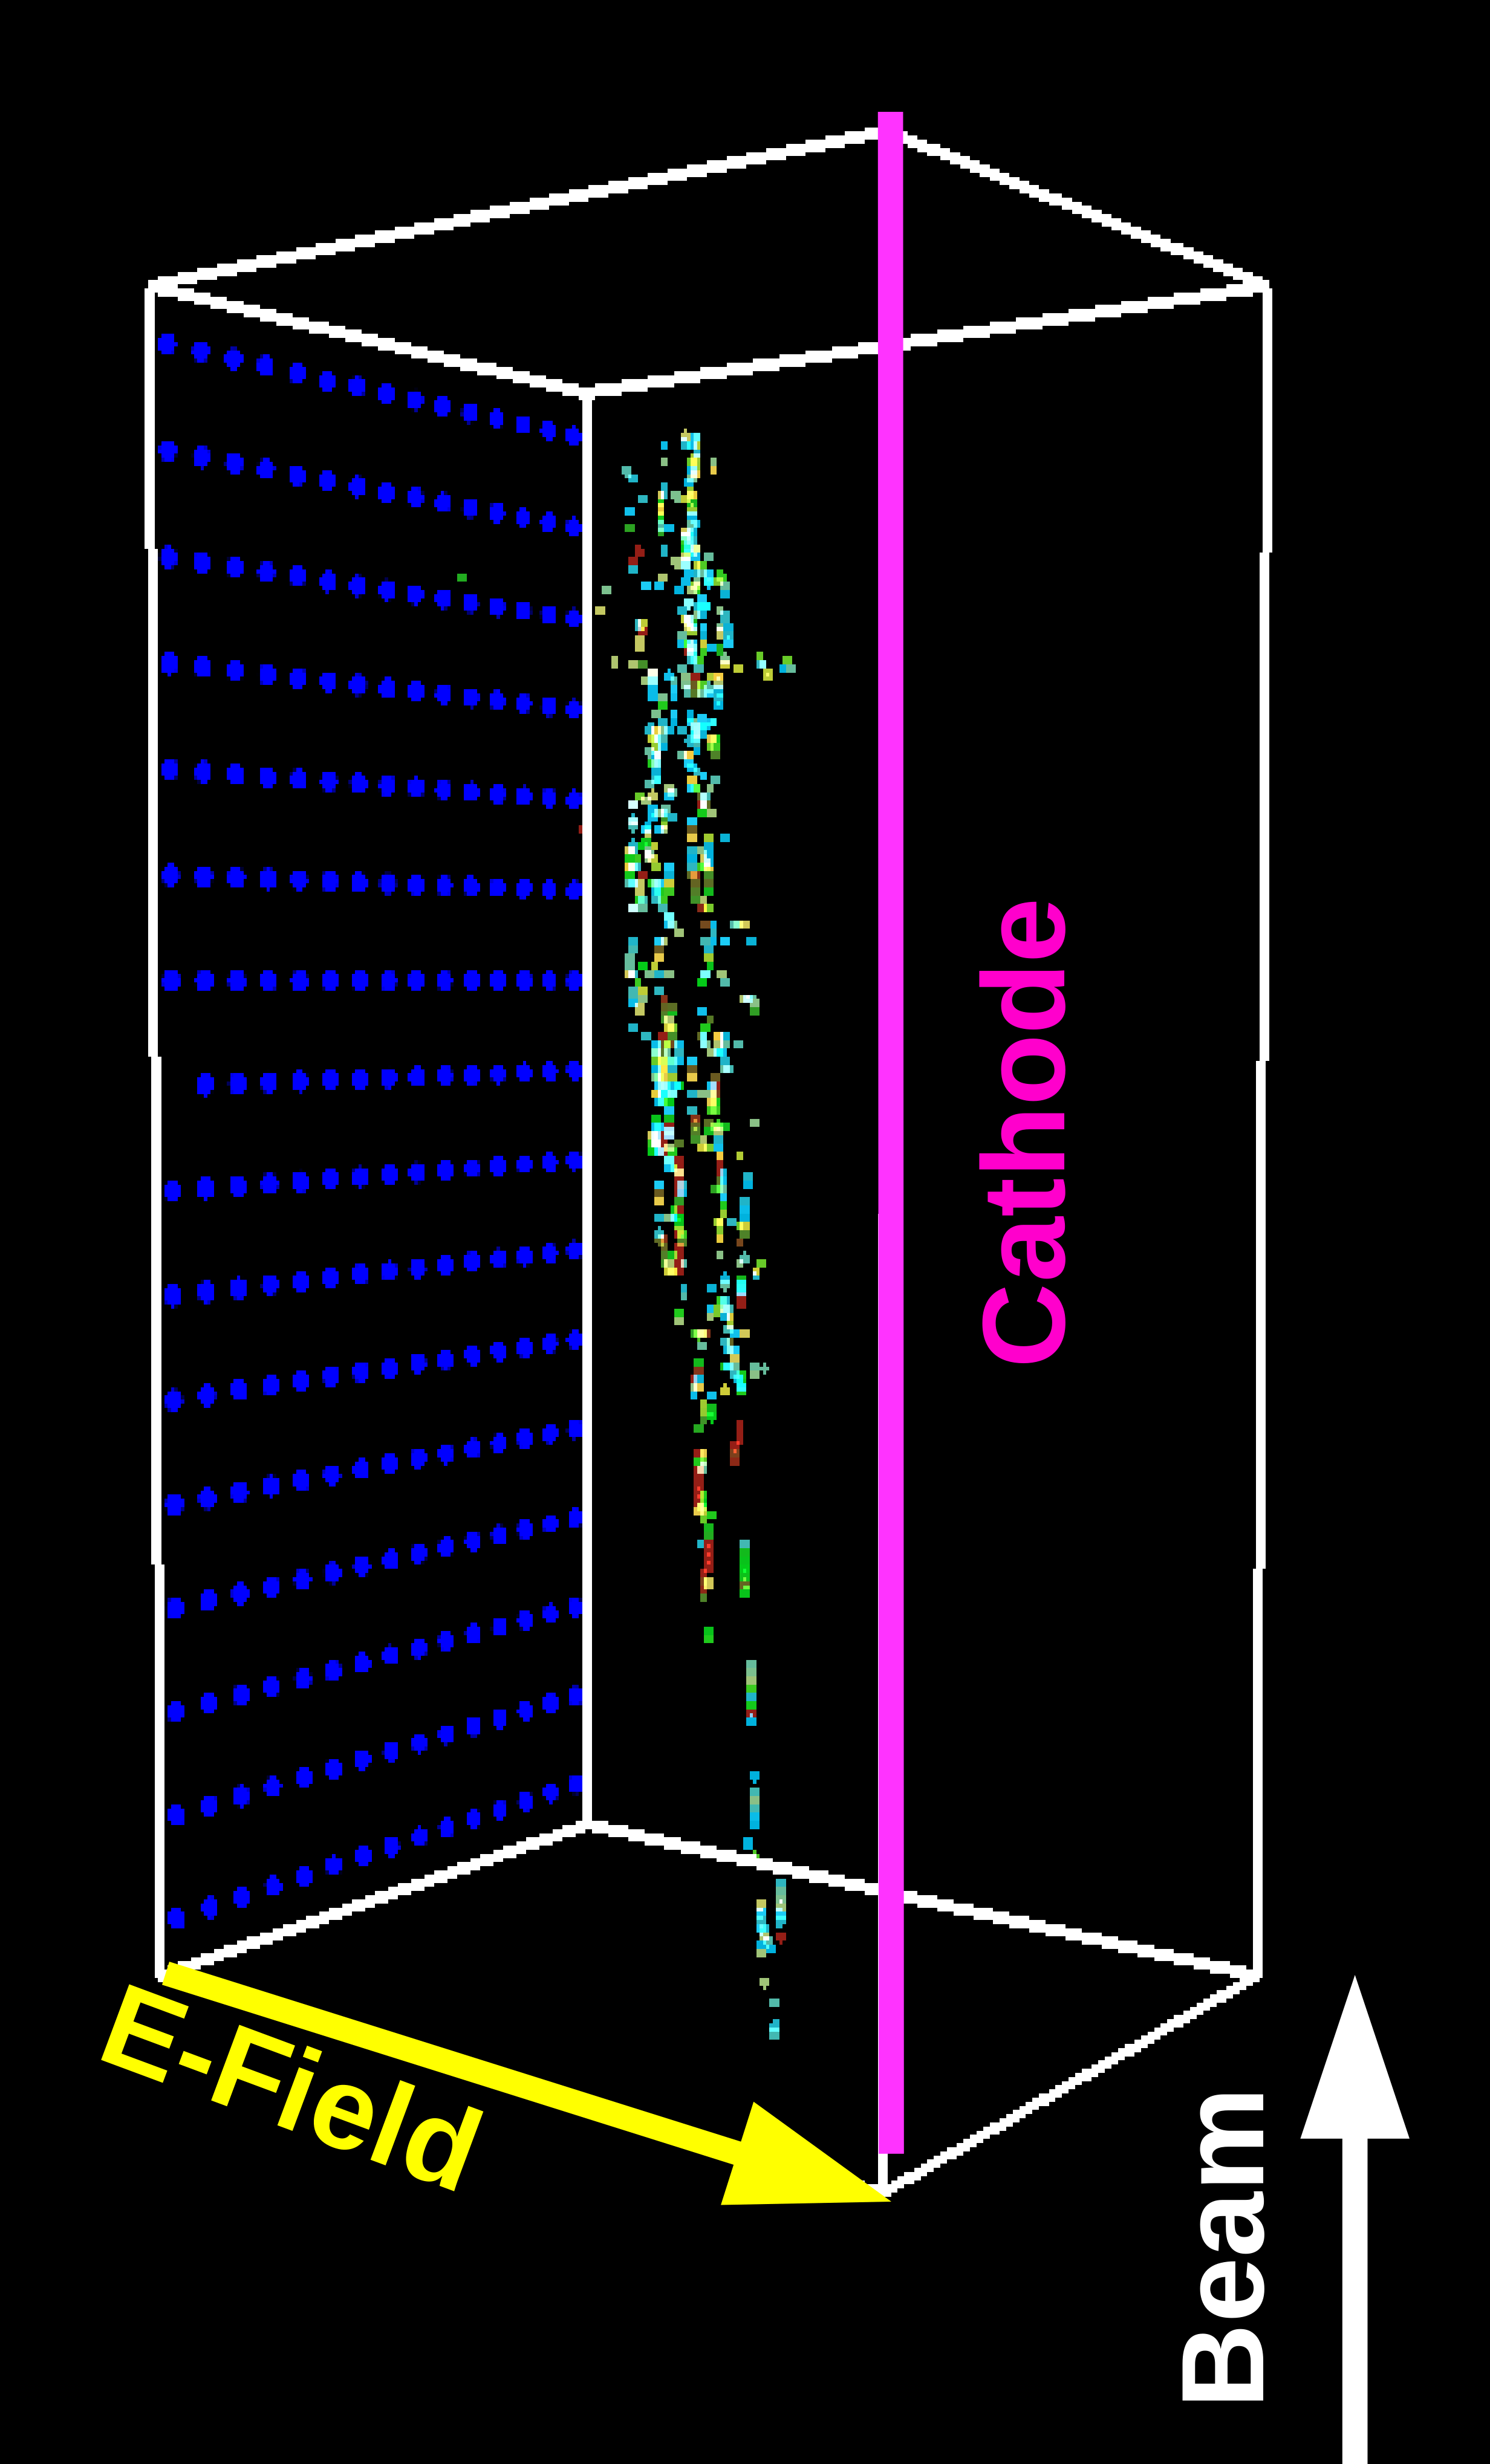
\includegraphics[height=.51\textheight]{pixlar/pixlar_event_side}
	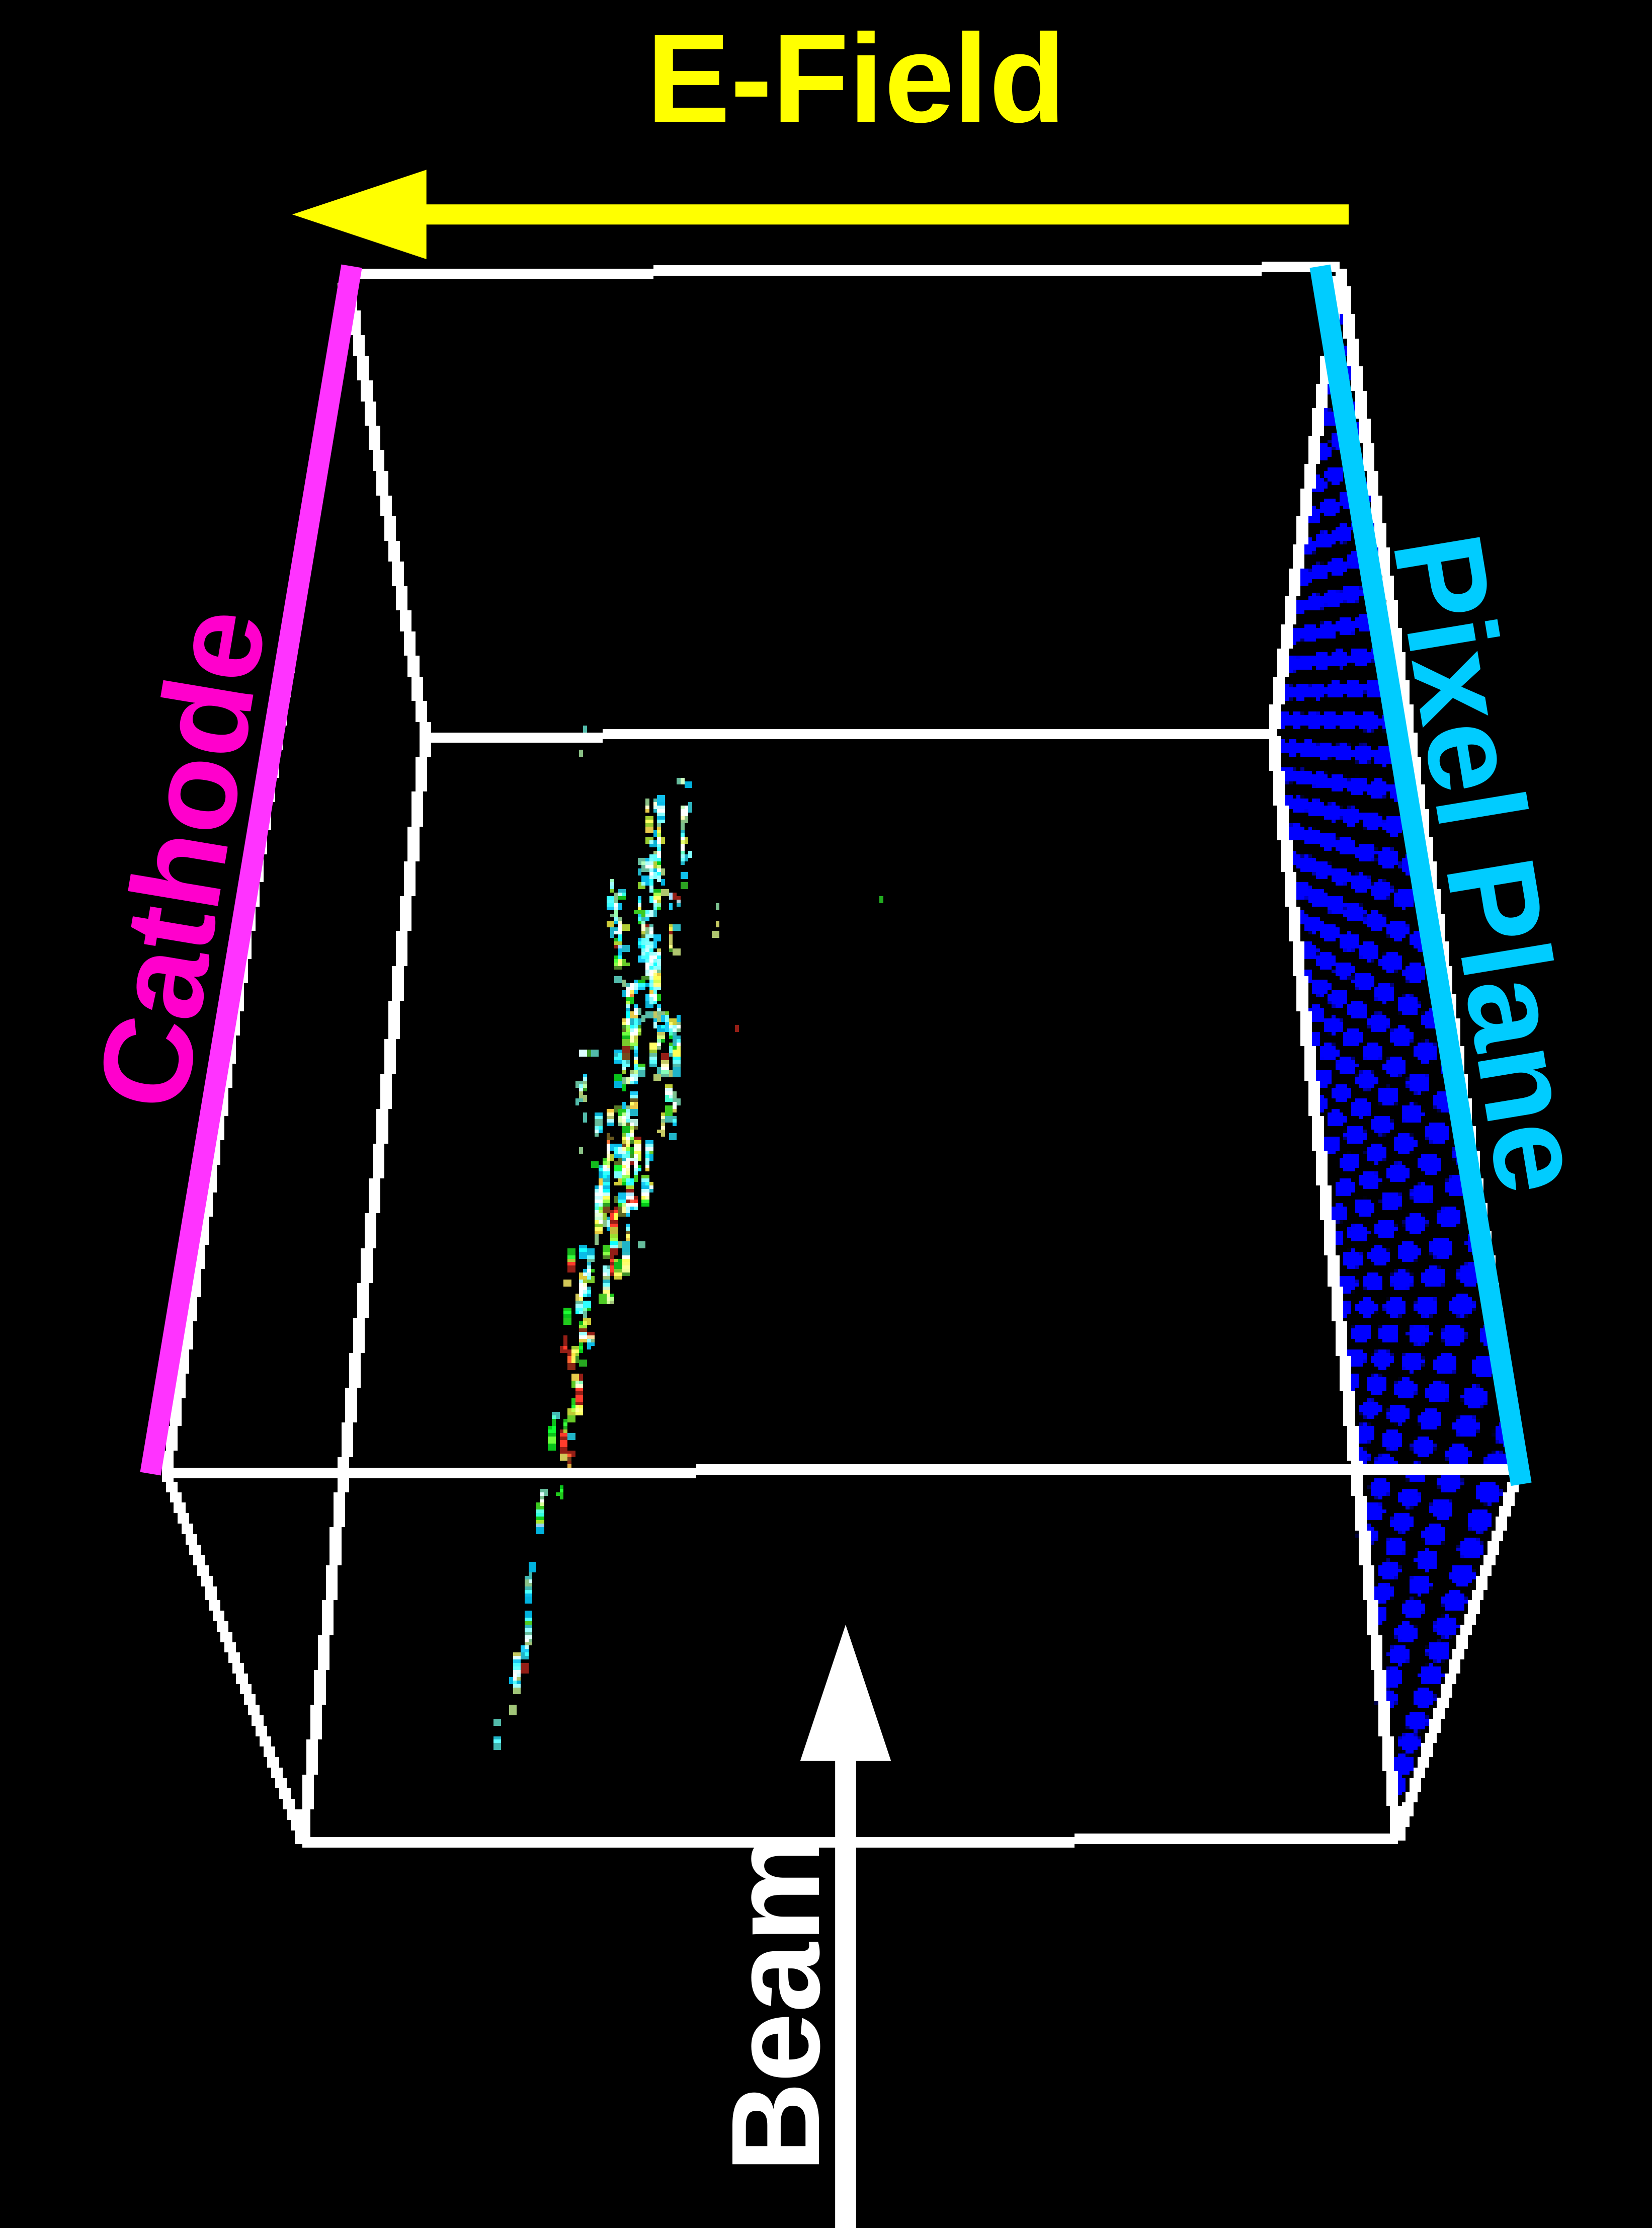
\includegraphics[height=.51\textheight]{pixlar/pixlar_event_top}
	\caption[\pixlar{} beam event]{%
		\pixlar{} beam event.
	}
	\label{fig:pixlar_event}
\end{figure}

Over several weeks beam and cosmic muon data was taken.
At the time of writing no official results were available.
Nevertheless, preliminary analyses indicate a successful scale-up of the pixelated \lartpc{} concept.
The achieved \gls{snr} is comparable to what was reached with the prototype at \gls{help} (see Section~\ref{sec:ac_viper}).
A recorded beam event is shown in Figure~\ref{fig:pixlar_event}.